\documentclass[11pt,a4paper]{article}
\usepackage[utf8]{inputenc}
\usepackage[T1]{fontenc}
\usepackage[spanish,es-noshorthands]{babel}
\usepackage[left=2.4cm,right=2.4cm,top=2.4cm,bottom=2.2cm]{geometry}
\usepackage{newunicodechar,amsmath,amssymb}
\usepackage{longtable,array,colortbl,xcolor,float,graphicx,enumitem,fancyvrb,needspace,caption}
\usepackage[colorlinks=true,linkcolor=black,urlcolor=black]{hyperref}
\setcounter{secnumdepth}{3}\setcounter{tocdepth}{3}
\emergencystretch=3em
\sloppy
\captionsetup{font=small,labelfont=bf}
\renewcommand{\abstractname}{Resumen}
\renewcommand{\contentsname}{Índice}
\renewcommand{\listfigurename}{Figuras}
\newunicodechar{²}{\ensuremath{^{2}}}
\newunicodechar{Δ}{\ensuremath{\Delta}}
\newunicodechar{Π}{\ensuremath{\Pi}}
\newunicodechar{λ}{\ensuremath{\lambda}}
\newunicodechar{ρ}{\ensuremath{\rho}}
\newunicodechar{φ}{\ensuremath{\varphi}}
\newunicodechar{→}{\ensuremath{\rightarrow}}
\newunicodechar{∈}{\ensuremath{\in}}
\newunicodechar{−}{\ensuremath{-}}
\newunicodechar{√}{\ensuremath{\surd}}
\newunicodechar{∩}{\ensuremath{\cap}}
\newunicodechar{∪}{\ensuremath{\cup}}
\newunicodechar{≈}{\ensuremath{\approx}}
\newunicodechar{≡}{\ensuremath{\equiv}}
\newunicodechar{⊆}{\ensuremath{\subseteq}}
\newunicodechar{⋃}{\ensuremath{\bigcup}}
\newunicodechar{⋈}{\ensuremath{\bowtie}}

\title{\textbf{Informe: Diseño de la base de datos}\\[1ex]\large Generación automática de itinerarios turísticos\\Proyecto Astarship}
\author{\textbf{Equipo: HAVING Fe}\\Bases de Datos II \textperiodcentered{} Ingeniería de Software\\Curso 2026--2027}
\date{\textit{Borrador para revisión del equipo}}
\begin{document}
\begin{titlepage}
\centering\vspace*{4cm}
{\Huge\bfseries Informe: Diseño de la base de datos\par}
\vspace{1cm}{\Large Generación automática de itinerarios turísticos\par}
\vspace{.4cm}{\Large Proyecto Astarship\par}
\vspace{1.5cm}{\large\bfseries Equipo: HAVING Fe\par}
\vspace{1cm}{\large Bases de Datos II \textperiodcentered{} Ingeniería de Software\par Curso 2026--2027\par}
\end{titlepage}
\pagestyle{plain}
\begin{abstract}
El presente informe tiene como objetivo diseñar una base de datos para la gestión de la generación automática de itinerarios turísticos de una agencia de viajes. Se realizó un análisis de los requerimientos funcionales, no funcionales y de entorno del sistema, lo que permitió identificar con claridad los procesos de gestión de guías, turistas, atracciones, actividades, paquetes, itinerarios y las seis consultas analíticas que constituyen el criterio de evaluación. A partir de ello se elaboró un Modelo Conceptual Relacional-Extendido (MERX, versión 1.8.1) que muestra las entidades, atributos, interrelaciones y agregaciones críticas, junto con la especificación de las restricciones de integridad y el esquema lógico relacional derivado. Finalmente, se valoró la corrección del diseño mediante la extracción del cubrimiento minimal de dependencias funcionales, la descomposición en Tercera Forma Normal (3FN) y la comprobación de las propiedades de preservación de dependencias (PPDF) y de join sin pérdida (PLJ). Se concluye que el diseño es coherente y se recogen, de forma explícita, los puntos abiertos que deben cerrarse antes de la implementación física.
\end{abstract}
\newpage
\newpage
\tableofcontents
\newpage
\newpage
\section{Introducción}
Este informe tiene como propósito mostrar el proceso de análisis, diseño y valoración teórica de la base de datos correspondiente al proyecto «Astarship — generación automática de itinerarios turísticos», desarrollado por el equipo HAVING Fe en el marco de las asignaturas Bases de Datos II e Ingeniería de Software. En él se recoge el trabajo colaborativo orientado a establecer una especificación clara que garantice la correcta implementación de los procesos de almacenamiento, abarcando desde la gestión de los distintos actores (guías turísticos, jefe de operaciones, turistas y administrador) hasta la generación de itinerarios equilibrados bajo criterios de proporción por tipo, cobertura de categorías y cantidad total de actividades.

El documento inicia con un análisis y reformulación de los requerimientos funcionales, no funcionales (rendimiento, arquitectura desacoplada, patrones de diseño) y las restricciones técnicas y de entorno. Seguidamente se muestra el Modelo Conceptual Relacional-Extendido (MERX) para representar de forma estructurada las entidades, interrelaciones y agregaciones que conforman la lógica del proyecto, así como el esquema lógico relacional que se deriva de él. A continuación se detallan las restricciones de integridad detectadas, incluyendo la definición de llaves, referencias, dominios, nulabilidad y cardinalidades por interrelación. Finalmente se realiza una valoración del diseño mediante la extracción del cubrimiento minimal y su descomposición en 3FN, evaluando su completitud y pertinencia teórica, y se señalan las observaciones y puntos abiertos detectados durante el análisis.

\section{Análisis y reformulación enriquecedora de los requerimientos funcionales e informacionales del sistema}
Astarship es una aplicación web para una agencia de viajes que genera itinerarios turísticos de forma automática. El sistema administra el banco de actividades y atracciones, los paquetes turísticos en que se usan, los guías que las describen y validan, y los turistas que las recorren. La generación no es aleatoria: cada itinerario debe respetar criterios de equilibrio y conservar el orden de recorrido para poder analizar cómo se acumula el esfuerzo físico a lo largo del viaje. Quedan fuera del alcance pagos, facturación, reservas de transporte o alojamiento, mensajería entre usuarios e integraciones con servicios externos.

\subsubsection*{Actores del sistema}
{\footnotesize\setlength{\tabcolsep}{3pt}\renewcommand{\arraystretch}{1.15}
\begin{longtable}{|>{\raggedright\arraybackslash}p{3.78cm}|>{\raggedright\arraybackslash}p{11.98cm}|}
\hline
\rowcolor{gray!20} \textbf{Actor} & \textbf{Qué hace en el sistema} \\ \hline
\endhead
Guía turístico & Registra atracciones y actividades; clasifica por categoría y tipo y asigna nivel de esfuerzo a las actividades que él describió; genera itinerarios; atiende solicitudes de modificación. \\ \hline
Jefe de operaciones turísticas & Revisa y aprueba los itinerarios generados; puede ordenar la confección de otro bajo sus criterios. \\ \hline
Turista & Consulta los itinerarios que le asignan, registra sus visitas, valora la experiencia y solicita modificaciones. \\ \hline
Administrador & Evita actividades duplicadas e impide la asignación doble de itinerarios (ver PA-1 en la sección 5.4). \\ \hline
\end{longtable}}
\vspace{2pt}
Un mismo guía puede estar autorizado en unos paquetes y no en otros, y la autorización distingue entre \textbf{generar} y \textbf{validar} itinerarios.

\subsection{Requerimientos Funcionales}
\subsubsection{Actividades y atracciones}
{\footnotesize\setlength{\tabcolsep}{3pt}\renewcommand{\arraystretch}{1.15}
\begin{longtable}{|>{\raggedright\arraybackslash}p{1.28cm}|>{\raggedright\arraybackslash}p{11.28cm}|>{\raggedright\arraybackslash}p{2.98cm}|}
\hline
\rowcolor{gray!20} \textbf{ID} & \textbf{Requisito} & \textbf{Actor} \\ \hline
\endhead
RF-01 & Registrar una atracción. & Guía \\ \hline
RF-02 & Registrar una actividad e indicar en qué atracción se realiza. & Guía \\ \hline
RF-03 & Clasificar una actividad por \textbf{categoría}, solo sobre las actividades que el propio guía describió. & Guía \\ \hline
RF-04 & Clasificar una actividad por \textbf{tipo}: visita, excursión o taller. & Guía \\ \hline
RF-05 & Asignar el \textbf{nivel de esfuerzo físico}: bajo, medio o alto. & Guía \\ \hline
RF-06 & Impedir que se registren actividades duplicadas. & Administrador \\ \hline
RF-07 & Consultar y listar el banco de actividades y atracciones. & Todos \\ \hline
\end{longtable}}
\vspace{2pt}
\subsubsection{Paquetes turísticos, guías y turistas}
{\footnotesize\setlength{\tabcolsep}{3pt}\renewcommand{\arraystretch}{1.15}
\begin{longtable}{|>{\raggedright\arraybackslash}p{1.28cm}|>{\raggedright\arraybackslash}p{11.28cm}|>{\raggedright\arraybackslash}p{2.98cm}|}
\hline
\rowcolor{gray!20} \textbf{ID} & \textbf{Requisito} & \textbf{Actor} \\ \hline
\endhead
RF-08 & Registrar un paquete con identificador único, nombre, destino y la lista de categorías a cubrir. & — \\ \hline
RF-09 & Registrar en qué paquetes está autorizado cada guía, distinguiendo si puede generar, validar o ambas. & — \\ \hline
RF-10 & Registrar un turista con identificador único, nombre, edad, grupo de viaje y los paquetes en que está inscrito. & — \\ \hline
RF-11 & Registrar un guía con identificador único, nombre y especialidad. & — \\ \hline
RF-12 & Gestionar grupos de viaje y la pertenencia de turistas a ellos. & — \\ \hline
\end{longtable}}
\vspace{2pt}
\subsubsection{Generación de itinerarios}
{\footnotesize\setlength{\tabcolsep}{3pt}\renewcommand{\arraystretch}{1.15}
\begin{longtable}{|>{\raggedright\arraybackslash}p{1.28cm}|>{\raggedright\arraybackslash}p{11.28cm}|>{\raggedright\arraybackslash}p{2.98cm}|}
\hline
\rowcolor{gray!20} \textbf{ID} & \textbf{Requisito} & \textbf{Actor} \\ \hline
\endhead
RF-13 & Generar un itinerario automáticamente a partir de un conjunto de actividades seleccionadas. & Guía autorizado \\ \hline
RF-14 & Parametrizar la generación con la proporción de actividades por tipo, la cobertura de categorías y la cantidad total de actividades. & Guía autorizado \\ \hline
RF-15 & Almacenar la parametrización junto al itinerario generado. & Sistema \\ \hline
RF-16 & Conservar el orden en que las actividades serán recorridas. & Sistema \\ \hline
RF-17 & Asociar cada itinerario a un paquete turístico. & Sistema \\ \hline
RF-18 & Consultar los itinerarios de otros guías que atienden el mismo paquete. & Guía \\ \hline
\end{longtable}}
\vspace{2pt}
El enunciado separa quién \textit{añade} actividades de quién \textit{crea} el itinerario: son roles distintos sobre la misma entidad Guía, no personas de distinto tipo.

\subsubsection{Validación}
{\footnotesize\setlength{\tabcolsep}{3pt}\renewcommand{\arraystretch}{1.15}
\begin{longtable}{|>{\raggedright\arraybackslash}p{1.28cm}|>{\raggedright\arraybackslash}p{11.28cm}|>{\raggedright\arraybackslash}p{2.98cm}|}
\hline
\rowcolor{gray!20} \textbf{ID} & \textbf{Requisito} & \textbf{Actor} \\ \hline
\endhead
RF-19 & Revisar y aprobar o rechazar un itinerario generado, registrando fecha de validación, resultado y observaciones. & Jefe de operaciones \\ \hline
RF-20 & Indicar la confección de otro itinerario bajo sus propios criterios. & Jefe de operaciones \\ \hline
RF-21 & Distinguir el estado de un itinerario entre «generado pendiente de validación» y «validado». & Sistema \\ \hline
\end{longtable}}
\vspace{2pt}
\subsubsection{Asignación y recorrido}
{\footnotesize\setlength{\tabcolsep}{3pt}\renewcommand{\arraystretch}{1.15}
\begin{longtable}{|>{\raggedright\arraybackslash}p{1.28cm}|>{\raggedright\arraybackslash}p{11.28cm}|>{\raggedright\arraybackslash}p{2.98cm}|}
\hline
\rowcolor{gray!20} \textbf{ID} & \textbf{Requisito} & \textbf{Actor} \\ \hline
\endhead
RF-22 & Asignar un itinerario a un turista (actor por definir, ver PA-1). & — \\ \hline
RF-23 & Impedir la asignación doble de itinerarios. & Administrador \\ \hline
RF-24 & Consultar los itinerarios asignados. & Turista \\ \hline
RF-25 & Registrar cada visita de un turista a una actividad de un itinerario recorrido. & Turista / Sistema \\ \hline
RF-26 & Valorar la experiencia. & Turista \\ \hline
RF-27 & Consultar las valoraciones. & Guía y Turista \\ \hline
RF-28 & Consultar todas las valoraciones propias agrupadas por paquete turístico. & Turista \\ \hline
\end{longtable}}
\vspace{2pt}
\subsubsection{Solicitud de modificación}
{\footnotesize\setlength{\tabcolsep}{3pt}\renewcommand{\arraystretch}{1.15}
\begin{longtable}{|>{\raggedright\arraybackslash}p{1.28cm}|>{\raggedright\arraybackslash}p{11.28cm}|>{\raggedright\arraybackslash}p{2.98cm}|}
\hline
\rowcolor{gray!20} \textbf{ID} & \textbf{Requisito} & \textbf{Actor} \\ \hline
\endhead
RF-29 & Solicitar de forma virtual una modificación del itinerario. & Turista \\ \hline
RF-30 & Pedir el apoyo de un guía adicional al asignado para que atienda la solicitud. & Turista \\ \hline
RF-31 & Registrar todo el proceso de solicitud y el resultado de la modificación manual. & Sistema \\ \hline
\end{longtable}}
\vspace{2pt}
\subsubsection{Red de atracciones}
{\footnotesize\setlength{\tabcolsep}{3pt}\renewcommand{\arraystretch}{1.15}
\begin{longtable}{|>{\raggedright\arraybackslash}p{1.28cm}|>{\raggedright\arraybackslash}p{11.28cm}|>{\raggedright\arraybackslash}p{2.98cm}|}
\hline
\rowcolor{gray!20} \textbf{ID} & \textbf{Requisito} & \textbf{Actor} \\ \hline
\endhead
RF-32 & Mantener las conexiones entre atracciones según cercanía geográfica y transporte disponible, con tiempo y costo asociados. & Sistema \\ \hline
RF-33 & Recorrer la red para proponer alternativas cuando una actividad no pueda realizarse en el horario previsto (Dijkstra con Strategy; ver sección 3.5). & Sistema \\ \hline
\end{longtable}}
\vspace{2pt}
\subsubsection{Reportes y exportación}
{\footnotesize\setlength{\tabcolsep}{3pt}\renewcommand{\arraystretch}{1.15}
\begin{longtable}{|>{\raggedright\arraybackslash}p{1.28cm}|>{\raggedright\arraybackslash}p{11.28cm}|>{\raggedright\arraybackslash}p{2.98cm}|}
\hline
\rowcolor{gray!20} \textbf{ID} & \textbf{Requisito} & \textbf{Actor} \\ \hline
\endhead
RF-34 & Generar reportes sobre la creación de itinerarios, las actividades más utilizadas, la distribución de niveles de esfuerzo y el desempeño de la experiencia según el esfuerzo. & Todos \\ \hline
RF-35 & Presentar los resultados en tablas y gráficos. & Sistema \\ \hline
RF-36 & Exportar a PDF la información mostrada, para todo tipo de usuario. & Todos \\ \hline
RF-37 & Ordenar cada columna de los resultados. & Todos \\ \hline
\end{longtable}}
\vspace{2pt}
\subsubsection{Consultas (criterio de evaluación)}
Técnicamente son requisitos funcionales; se separan porque constituyen el criterio de evaluación de Bases de Datos. Cada una debe poder verse como tabla y como gráfico, exportarse a PDF y ordenarse por columna (RF-35 a RF-37).

{\footnotesize\setlength{\tabcolsep}{3pt}\renewcommand{\arraystretch}{1.15}
\begin{longtable}{|>{\raggedright\arraybackslash}p{1.28cm}|>{\raggedright\arraybackslash}p{14.48cm}|}
\hline
\rowcolor{gray!20} \textbf{ID} & \textbf{Consulta} \\ \hline
\endhead
RC-1 & Itinerarios generados automáticamente para un paquete, indicando creador, fecha de creación y parámetros utilizados. \\ \hline
RC-2 & Actividades más utilizadas en los itinerarios finales de un paquete, clasificadas por nivel de esfuerzo y categoría. \\ \hline
RC-3 & Itinerarios validados por un revisor determinado, con fecha de validación y observaciones. \\ \hline
RC-4 & Experiencia de los turistas en un itinerario, clasificando las actividades por esfuerzo y comparando tasas de satisfacción. \\ \hline
RC-5 & Comparación entre paquetes: distribución de actividades por categoría y esfuerzo, y cumplimiento de los criterios de equilibrio. \\ \hline
RC-6 & Correlación entre nivel de esfuerzo y valoración promedio por paquete; las 10 actividades con mayor tasa de abandono (con su guía creador y su paquete); y la comparación del desempeño de los turistas que solicitaron modificación contra el promedio de sus grupos de viaje en esos mismos paquetes. \\ \hline
\end{longtable}}
\vspace{2pt}
RC-6 es la consulta más exigente y condiciona el modelo: exige calcular una \textit{tasa de abandono} por actividad (distinguir una visita realizada de una no realizada, RF-25), trazar cada actividad hasta el guía que la creó (RF-02) y relacionar solicitudes de modificación con valoraciones y grupos de viaje.

\subsection{Requerimientos No Funcionales}
{\footnotesize\setlength{\tabcolsep}{3pt}\renewcommand{\arraystretch}{1.15}
\begin{longtable}{|>{\raggedright\arraybackslash}p{1.48cm}|>{\raggedright\arraybackslash}p{14.28cm}|}
\hline
\rowcolor{gray!20} \textbf{ID} & \textbf{Requisito} \\ \hline
\endhead
RNF-01 & \textbf{Rendimiento.} El itinerario del día debe entregarse sin demoras perceptibles, incluso con varios grupos consultando a la vez; justifica una capa de caché. \\ \hline
RNF-02 & \textbf{La red de atracciones no se modela como tabla del esquema relacional.} Se gestiona de forma independiente para poder navegarla con agilidad. \\ \hline
RNF-03 & \textbf{Multiplataforma.} Accesible desde cualquier sistema; una aplicación web es suficiente. \\ \hline
RNF-04 & \textbf{Arquitectura desacoplada, extensible y mantenible.} \\ \hline
RNF-05 & \textbf{Patrones de diseño.} Al menos dos implementados y justificados (Strategy para el algoritmo de rutas, sección 3.5). \\ \hline
RNF-06 & \textbf{Documentación.} Docstrings en todo el código, verificados automáticamente. \\ \hline
RNF-07 & \textbf{Pruebas unitarias} de back-end y front-end. \\ \hline
RNF-08 & \textbf{Control de versiones} (Git + GitHub). \\ \hline
RNF-09 & \textbf{Planificación} con herramienta CASE. \\ \hline
RNF-10 & \textbf{Autenticación y autorización por rol.} Cada actor ve y hace solo lo que le corresponde. \\ \hline
\end{longtable}}
\vspace{2pt}
\subsection{Requerimientos de Entorno}
Decisiones técnicas ya tomadas por el equipo y aprobadas por el profesor:

\begin{itemize}[leftmargin=1.2em,itemsep=2pt,topsep=3pt]
\item \textbf{RE-01 Backend:} Python + FastAPI, gestionado con \texttt{uv}.
\item \textbf{RE-02 Base de datos:} PostgreSQL 18, con SQLAlchemy y migraciones con Alembic.
\item \textbf{RE-03 Frontend:} TypeScript + React (Vite).
\item \textbf{RE-04 Entorno:} Docker y Docker Compose.
\item \textbf{RE-05 Despliegue:} propuesto Vercel (frontend) + Render (API); sin cerrar.
\item \textbf{RE-06 Caché:} Redis, si RNF-01 lo exige.
\end{itemize}
\newpage
\section{Modelo Conceptual Relacional-Extendido (MERX)}
El MERX (versión 1.8.1) se organiza en tres bloques: entidades con sus atributos, interrelaciones binarias y agregaciones que modelan las interrelaciones con atributos propios o que participan en otras interrelaciones.

\subsection{Entidades}
\begin{figure}[H]\centering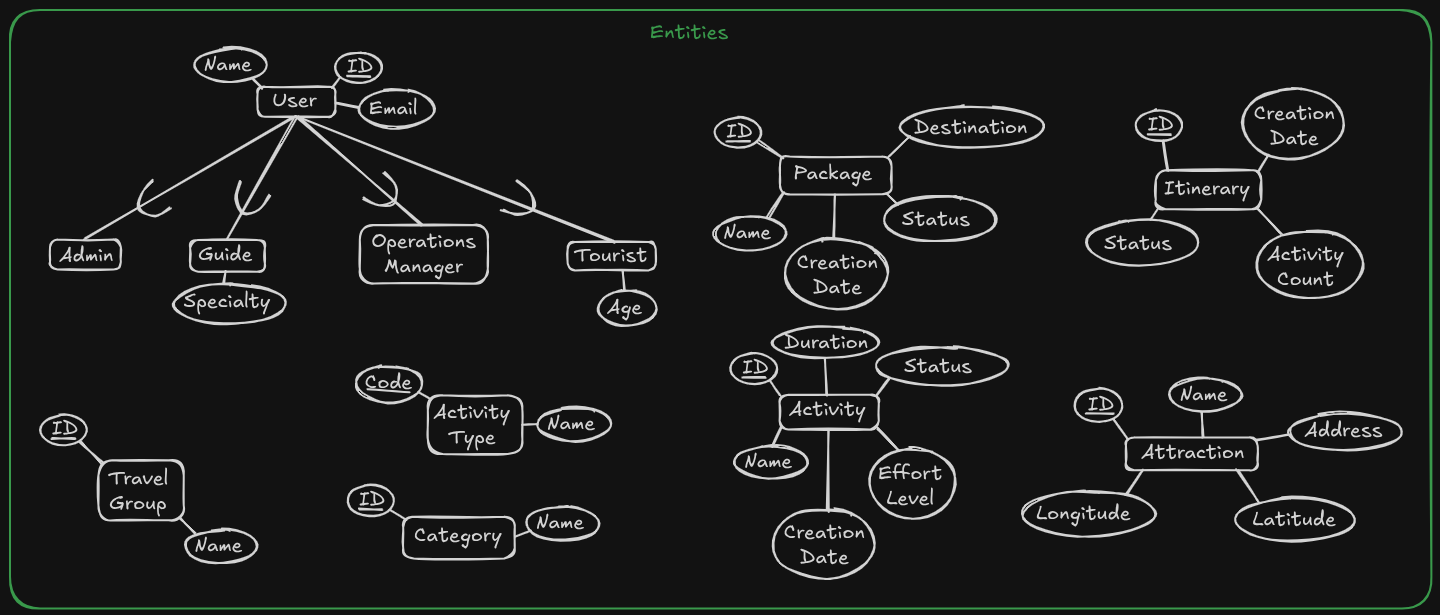
\includegraphics[width=16.20cm]{ent.png}\caption{MERX v1.8.1 — Entidades.}\end{figure}
{\footnotesize\setlength{\tabcolsep}{3pt}\renewcommand{\arraystretch}{1.15}
\begin{longtable}{|>{\raggedright\arraybackslash}p{3.28cm}|>{\raggedright\arraybackslash}p{12.48cm}|}
\hline
\rowcolor{gray!20} \textbf{Entidad} & \textbf{Atributos} \\ \hline
\endhead
User & \underline{ID}, Name, Email \\ \hline
TravelGroup & \underline{ID}, Name \\ \hline
Package & \underline{ID}, Name, Destination, Status, CreationDate \\ \hline
Itinerary & \underline{ID}, CreationDate, Status, ActivityCount \\ \hline
ActivityType & \underline{Code}, Name \\ \hline
Category & \underline{ID}, Name \\ \hline
Activity & \underline{ID}, Name, EffortLevel, Duration, Status, CreationDate \\ \hline
Attraction & \underline{ID}, Name, Address, Latitude, Longitude \\ \hline
\end{longtable}}
\vspace{2pt}
\textbf{Especialización de User} (total, disjunta — partición):

{\footnotesize\setlength{\tabcolsep}{3pt}\renewcommand{\arraystretch}{1.15}
\begin{longtable}{|>{\raggedright\arraybackslash}p{3.28cm}|>{\raggedright\arraybackslash}p{4.28cm}|>{\raggedright\arraybackslash}p{7.98cm}|}
\hline
\rowcolor{gray!20} \textbf{Supertipo} & \textbf{Subtipo} & \textbf{Atributos propios} \\ \hline
\endhead
User & Admin & — \\ \hline
User & Guide & Specialty \\ \hline
User & OperationsManager & — \\ \hline
User & Tourist & Age \\ \hline
\end{longtable}}
\vspace{2pt}
\needspace{8\baselineskip}
\subsection{Interrelaciones}
\begin{figure}[H]\centering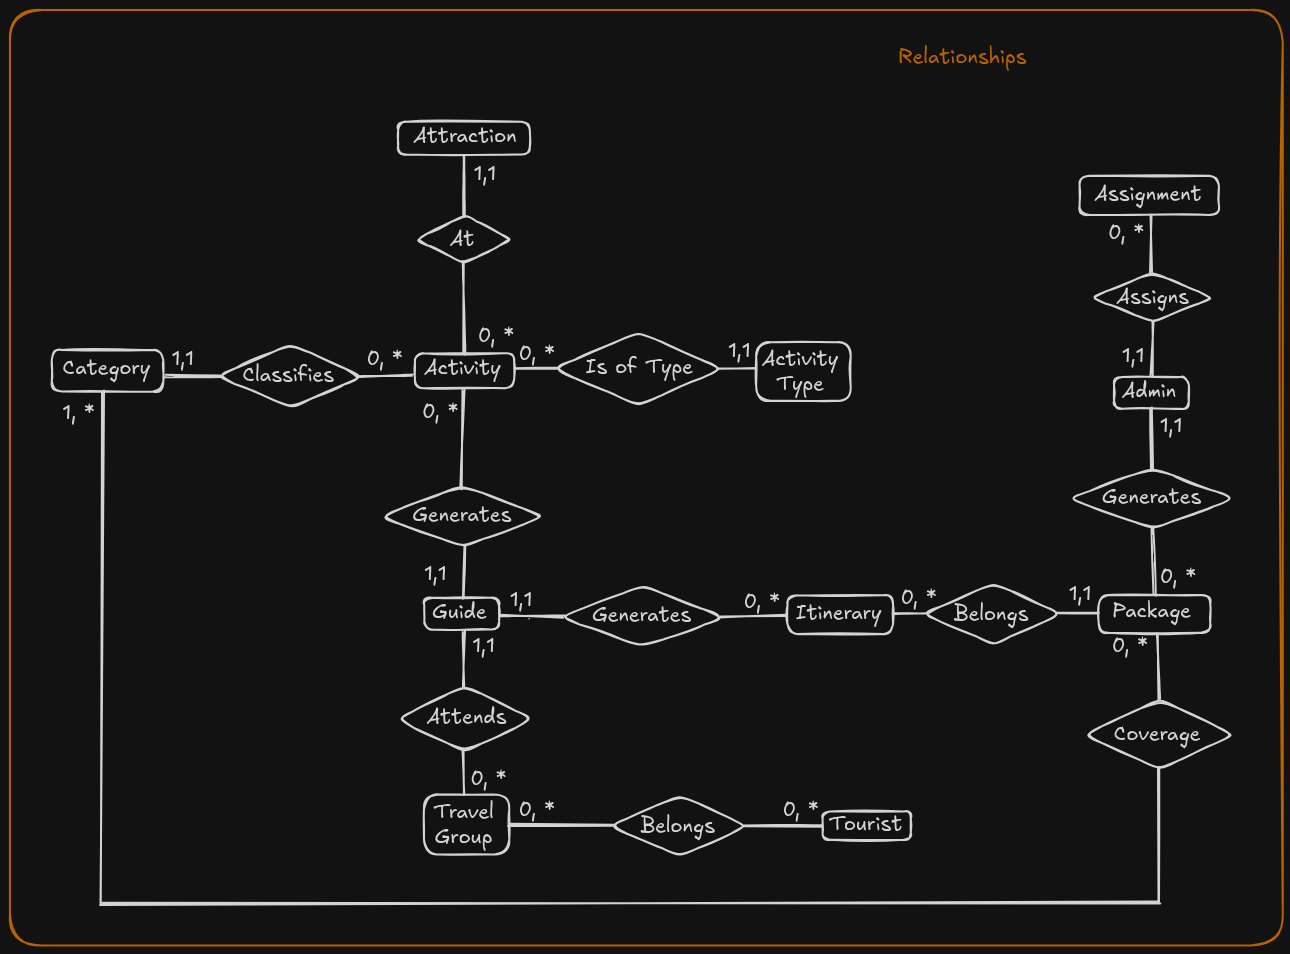
\includegraphics[width=12.60cm]{rel.png}\caption{MERX v1.8.1 — Interrelaciones.}\end{figure}
{\footnotesize\setlength{\tabcolsep}{3pt}\renewcommand{\arraystretch}{1.15}
\begin{longtable}{|>{\raggedright\arraybackslash}p{2.48cm}|>{\raggedright\arraybackslash}p{4.08cm}|>{\raggedright\arraybackslash}p{2.38cm}|>{\raggedright\arraybackslash}p{6.38cm}|}
\hline
\rowcolor{gray!20} \textbf{Interrelación} & \textbf{Participantes} & \textbf{Cardinalidad} & \textbf{(min,max)} \\ \hline
\endhead
Belongs & Tourist — TravelGroup & N:1 & Tourist (1,1) — TravelGroup (1,*) \\ \hline
Classifies & Activity — Category & N:1 & Activity (1,1) — Category (0,*) \\ \hline
Is of Type & Activity — ActivityType & N:1 & Activity (1,1) — ActivityType (0,*) \\ \hline
Coverage & Category — Package & N:M & Category (0,*) — Package (1,*) \\ \hline
Generates & Activity — Guide & N:1 & Activity (1,1) — Guide (0,*) \\ \hline
At & Activity — Attraction & N:1 & Activity (1,1) — Attraction (0,*) \\ \hline
Attends & Guide — TravelGroup & 1:N & Guide (0,*) — TravelGroup (1,1) \\ \hline
Belongs & Itinerary — Package & N:1 & Itinerary (1,1) — Package (0,*) \\ \hline
Generates & Package — Admin & N:1 & Package (1,1) — Admin (0,*) \\ \hline
Generates & Itinerary — Guide & N:1 & Itinerary (1,1) — Guide (0,*) \\ \hline
Assigns & Admin — Assignment & 1:N & Admin (0,*) — Assignment (1,1) \\ \hline
\end{longtable}}
\vspace{2pt}
\newpage
\subsection{Agregaciones}
\begin{figure}[H]\centering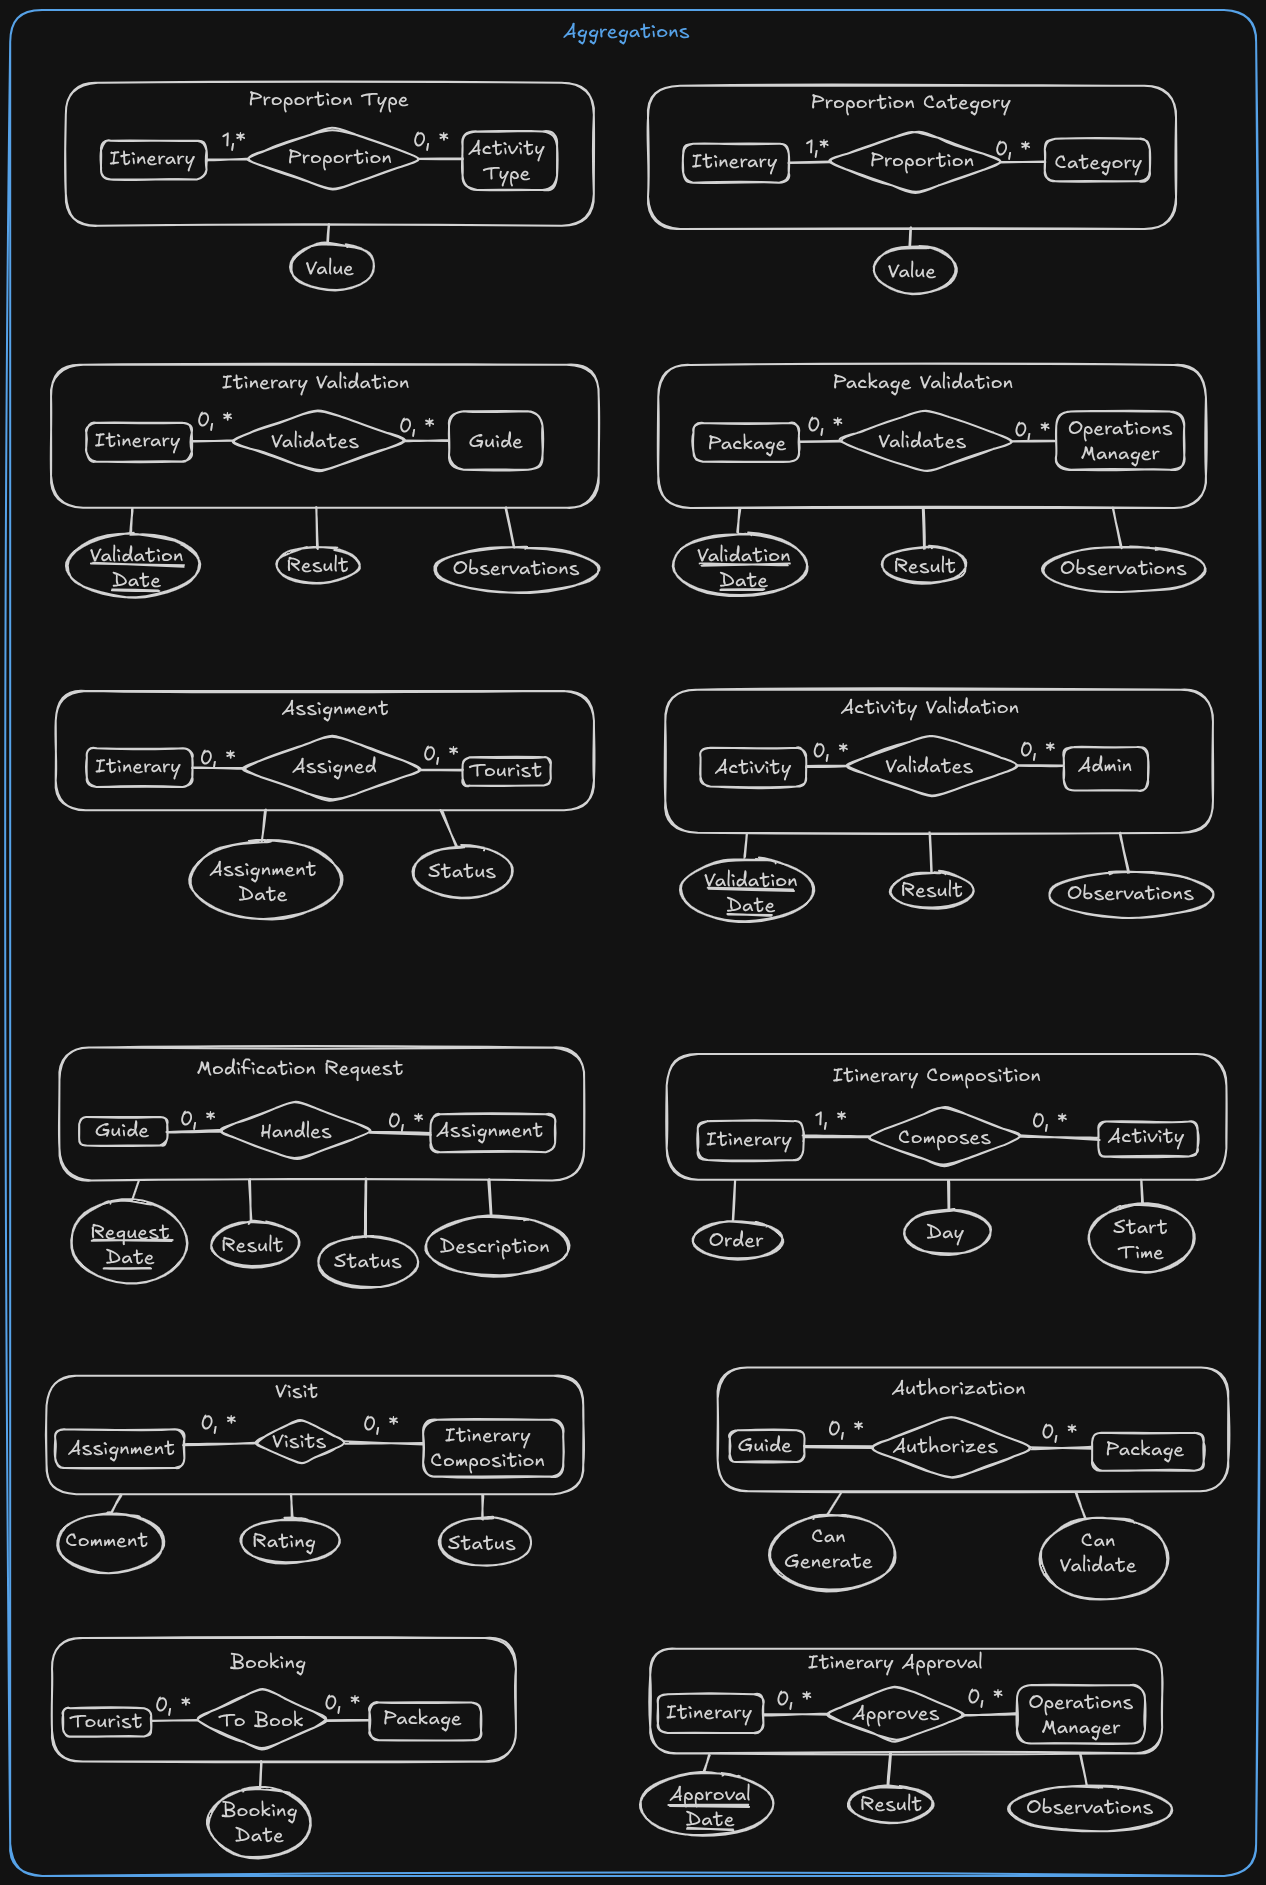
\includegraphics[width=13.57cm]{agg.png}\caption{MERX v1.8.1 — Agregaciones.}\end{figure}
{\footnotesize\setlength{\tabcolsep}{3pt}\renewcommand{\arraystretch}{1.15}
\begin{longtable}{|>{\raggedright\arraybackslash}p{2.68cm}|>{\raggedright\arraybackslash}p{3.28cm}|>{\raggedright\arraybackslash}p{0.88cm}|>{\raggedright\arraybackslash}p{4.18cm}|>{\raggedright\arraybackslash}p{4.08cm}|}
\hline
\rowcolor{gray!20} \textbf{Agregación} & \textbf{Participantes} & \textbf{Card.} & \textbf{(min,max)} & \textbf{Atributos} \\ \hline
\endhead
Proportion Type & Itinerary — ActivityType & N:M & Itinerary (1,*) — ActivityType (0,*) & Value \\ \hline
Proportion Category & Itinerary — Category & N:M & Itinerary (1,*) — Category (0,*) & Value \\ \hline
Itinerary Validation & Itinerary — Guide & N:M & Itinerary (0,*) — Guide (0,*) & ValidationDate, Result, Observations \\ \hline
Itinerary Approval & Itinerary — OperationsManager & N:M & Itinerary (0,*) — OperationsManager (0,*) & ApprovalDate, Result, Observations \\ \hline
Package Validation & Package — OperationsManager & N:M & Package (0,*) — OperationsManager (0,*) & ValidationDate, Result, Observations \\ \hline
Activity Validation & Activity — Admin & N:M & Activity (0,*) — Admin (0,*) & ValidationDate, Result, Observations \\ \hline
Assignment & Itinerary — Tourist & N:M & Itinerary (0,*) — Tourist (0,*) & AssignmentDate, Status \\ \hline
Modification Request & Guide — Assignment & N:M & Guide (0,*) — Assignment (0,*) & RequestDate, Description, Status, Result \\ \hline
Itinerary Composition & Itinerary — Activity & N:M & Itinerary (1,*) — Activity (0,*) & Order, Day, StartTime \\ \hline
Visit & Assignment — Itinerary Composition & N:M & Assignment (0,*) — Itinerary Composition (0,*) & Comment, Rating, Status \\ \hline
Authorization & Guide — Package & N:M & Guide (0,*) — Package (0,*) & CanGenerate, CanValidate \\ \hline
Booking & Tourist — Package & N:M & Tourist (0,*) — Package (0,*) & BookingDate \\ \hline
\end{longtable}}
\vspace{2pt}
Las agregaciones \textit{Assignment} e \textit{Itinerary Composition} participan a su vez como extremos de otras interrelaciones (\textit{Modification Request} y \textit{Visit}), por lo que se tratan como entidades agregadas con identidad propia dada por la concatenación de las llaves de sus participantes.

\needspace{8\baselineskip}
\subsection{Esquema lógico relacional}
Aplicando las reglas de transformación del MERX al modelo relacional se obtienen 25 esquemas: las entidades incorporan como llave foránea las interrelaciones de cardinalidad N:1 / 1:N; cada subtipo de la especialización comparte la llave de User (partición total y disjunta); la interrelación N:M Coverage y las agregaciones generan esquemas propios cuya llave es la concatenación de las llaves de sus participantes.

{\footnotesize\setlength{\tabcolsep}{3pt}\renewcommand{\arraystretch}{1.15}
\begin{longtable}{|>{\raggedright\arraybackslash}p{2.88cm}|>{\raggedright\arraybackslash}p{1.78cm}|>{\raggedright\arraybackslash}p{5.38cm}|>{\raggedright\arraybackslash}p{5.28cm}|}
\hline
\rowcolor{gray!20} \textbf{Relación} & \textbf{Tipo} & \textbf{Atributos (llave subrayada)} & \textbf{Llaves foráneas} \\ \hline
\endhead
User & Entidad & \underline{ID}, Name, Email & — \\ \hline
TravelGroup & Entidad & \underline{ID}, Name, ID\_Guide & (ID\_Guide) \ensuremath{\rightarrow} Guide(ID) \\ \hline
Package & Entidad & \underline{ID}, Name, Destination, Status, CreationDate, ID\_Admin & (ID\_Admin) \ensuremath{\rightarrow} Admin(ID) \\ \hline
Itinerary & Entidad & \underline{ID}, CreationDate, Status, ActivityCount, ID\_Package, ID\_Guide & (ID\_Package) \ensuremath{\rightarrow} Package(ID)\newline{}(ID\_Guide) \ensuremath{\rightarrow} Guide(ID) \\ \hline
ActivityType & Entidad & \underline{Code}, Name & — \\ \hline
Category & Entidad & \underline{ID}, Name & — \\ \hline
Attraction & Entidad & \underline{ID}, Name, Address, Latitude, Longitude & — \\ \hline
Activity & Entidad & \underline{ID}, Name, EffortLevel, Duration, Status, CreationDate, Code\_Type, ID\_Category, ID\_Guide, ID\_Attraction & (Code\_Type) \ensuremath{\rightarrow} ActivityType(Code)\newline{}(ID\_Category) \ensuremath{\rightarrow} Category(ID)\newline{}(ID\_Guide) \ensuremath{\rightarrow} Guide(ID)\newline{}(ID\_Attraction) \ensuremath{\rightarrow} Attraction(ID) \\ \hline
Admin & Especialización & \underline{ID} & (ID) \ensuremath{\rightarrow} User(ID) \\ \hline
Guide & Especialización & \underline{ID}, Specialty & (ID) \ensuremath{\rightarrow} User(ID) \\ \hline
OperationsManager & Especialización & \underline{ID} & (ID) \ensuremath{\rightarrow} User(ID) \\ \hline
Tourist & Especialización & \underline{ID}, Age, ID\_TravelGroup & (ID) \ensuremath{\rightarrow} User(ID)\newline{}(ID\_TravelGroup) \ensuremath{\rightarrow} TravelGroup(ID) \\ \hline
Coverage & Interrelación & \underline{ID\_Package}, \underline{ID\_Category} & (ID\_Package) \ensuremath{\rightarrow} Package(ID)\newline{}(ID\_Category) \ensuremath{\rightarrow} Category(ID) \\ \hline
ProportionType & Agregación & \underline{ID\_Itinerary}, \underline{Code\_Type}, Value & (ID\_Itinerary) \ensuremath{\rightarrow} Itinerary(ID)\newline{}(Code\_Type) \ensuremath{\rightarrow} ActivityType(Code) \\ \hline
ProportionCategory & Agregación & \underline{ID\_Itinerary}, \underline{ID\_Category}, Value & (ID\_Itinerary) \ensuremath{\rightarrow} Itinerary(ID)\newline{}(ID\_Category) \ensuremath{\rightarrow} Category(ID) \\ \hline
ItineraryValidation & Agregación & \underline{ID\_Itinerary}, \underline{ID\_Guide}, \underline{ValidationDate}, Result, Observations & (ID\_Itinerary) \ensuremath{\rightarrow} Itinerary(ID)\newline{}(ID\_Guide) \ensuremath{\rightarrow} Guide(ID) \\ \hline
ItineraryApproval & Agregación & \underline{ID\_Itinerary}, \underline{ID\_Manager}, \underline{ApprovalDate}, Result, Observations & (ID\_Itinerary) \ensuremath{\rightarrow} Itinerary(ID)\newline{}(ID\_Manager) \ensuremath{\rightarrow} OperationsManager(ID) \\ \hline
PackageValidation & Agregación & \underline{ID\_Package}, \underline{ID\_Manager}, \underline{ValidationDate}, Result, Observations & (ID\_Package) \ensuremath{\rightarrow} Package(ID)\newline{}(ID\_Manager) \ensuremath{\rightarrow} OperationsManager(ID) \\ \hline
ActivityValidation & Agregación & \underline{ID\_Activity}, \underline{ID\_Admin}, \underline{ValidationDate}, Result, Observations & (ID\_Activity) \ensuremath{\rightarrow} Activity(ID)\newline{}(ID\_Admin) \ensuremath{\rightarrow} Admin(ID) \\ \hline
Assignment & Agregación & \underline{ID\_Itinerary}, \underline{ID\_Tourist}, AssignmentDate, Status, ID\_Admin & (ID\_Itinerary) \ensuremath{\rightarrow} Itinerary(ID)\newline{}(ID\_Tourist) \ensuremath{\rightarrow} Tourist(ID)\newline{}(ID\_Admin) \ensuremath{\rightarrow} Admin(ID) \\ \hline
ModificationRequest & Agregación & \underline{ID\_Itinerary}, \underline{ID\_Tourist}, \underline{ID\_Guide}, \underline{RequestDate}, Description, Status, Result & (ID\_Itinerary, ID\_Tourist) \ensuremath{\rightarrow} Assignment(ID\_Itinerary, ID\_Tourist)\newline{}(ID\_Guide) \ensuremath{\rightarrow} Guide(ID) \\ \hline
ItineraryComposition & Agregación & \underline{ID\_Itinerary}, \underline{ID\_Activity}, Order, Day, StartTime & (ID\_Itinerary) \ensuremath{\rightarrow} Itinerary(ID)\newline{}(ID\_Activity) \ensuremath{\rightarrow} Activity(ID) \\ \hline
Visit & Agregación & \underline{ID\_Itinerary}, \underline{ID\_Tourist}, \underline{ID\_Activity}, Comment, Rating, Status & (ID\_Itinerary, ID\_Tourist) \ensuremath{\rightarrow} Assignment(ID\_Itinerary, ID\_Tourist)\newline{}(ID\_Itinerary, ID\_Activity) \ensuremath{\rightarrow} ItineraryComposition(ID\_Itinerary, ID\_Activity) \\ \hline
Authorization & Agregación & \underline{ID\_Guide}, \underline{ID\_Package}, CanGenerate, CanValidate & (ID\_Guide) \ensuremath{\rightarrow} Guide(ID)\newline{}(ID\_Package) \ensuremath{\rightarrow} Package(ID) \\ \hline
Booking & Agregación & \underline{ID\_Tourist}, \underline{ID\_Package}, BookingDate & (ID\_Tourist) \ensuremath{\rightarrow} Tourist(ID)\newline{}(ID\_Package) \ensuremath{\rightarrow} Package(ID) \\ \hline
\end{longtable}}
\vspace{2pt}
Conforme a RNF-02, la red de atracciones (tiempos y costos entre atracciones) \textbf{no} forma parte de este esquema relacional: se gestiona de forma independiente y se enlaza con Attraction mediante su identificador.

\subsection{Red de atracciones y búsqueda de alternativas (RF-33)}
RF-33 exige recorrer la red de atracciones para proponer alternativas cuando una actividad no puede realizarse en el horario previsto. Por RNF-02 la red no vive en el esquema relacional: cada \textit{nodo} es una atracción (identificada por \texttt{Attraction.ID}, con \texttt{Latitude} y \texttt{Longitude}) y cada \textit{arista} es una conexión dirigida con dos pesos, \textbf{tiempo} y \textbf{costo} (RF-32). Esta subsección describe el algoritmo elegido y su integración en el sistema.

\subsubsection{Algoritmo base: Dijkstra}
Dijkstra encuentra el camino de menor peso acumulado entre un origen y un destino en un grafo dirigido con pesos no negativos. Mantiene una cola de prioridad ordenada por \textit{g(n)}, el peso acumulado desde el origen, y en cada paso extrae el nodo de menor \textit{g(n)} y relaja sus aristas salientes. Como los pesos (tiempo y costo, RF-32) son no negativos, la primera vez que un nodo sale de la cola su peso es el óptimo, por lo que la búsqueda puede detenerse al extraer el destino.

\begin{itemize}[leftmargin=1.2em,itemsep=2pt,topsep=3pt]
\item \textbf{Peso por tiempo y peso por costo.} El mismo algoritmo sirve para ambos criterios: solo cambia la función \textit{peso(arista)} que se le entrega (el tiempo o el costo de la conexión). No requiere coordenadas ni heurística, por lo que no depende de \texttt{Latitude} y \texttt{Longitude} de Attraction.
\item \textbf{Alternativas múltiples.} Una única ejecución desde la atracción de origen calcula el peso mínimo hacia \textit{todas} las atracciones alcanzables, de modo que el servicio puede evaluar todas las atracciones candidatas con una sola pasada en lugar de una búsqueda por candidata.
\item \textbf{Complejidad.} O((V + E) log V) con cola de prioridad binaria, siendo V el número de atracciones y E el de conexiones.
\end{itemize}

\begin{Verbatim}[fontsize=\scriptsize,frame=single,framesep=2mm]
DIJKSTRA(grafo, origen, destino, peso):
    abiertos <- cola_prioridad();  g[origen] <- 0
    abiertos.insertar(origen, prioridad = 0)
    mientras abiertos no vacia:
        n <- abiertos.extraer_minimo()
        si n == destino: devolver reconstruir_camino(padre, n)
        para cada arista (n, m, w) en grafo.vecinos(n):
            nuevo <- g[n] + peso(w)             # tiempo o costo
            si nuevo < g.get(m, infinito):
                g[m] <- nuevo;  padre[m] <- n
                abiertos.insertar_o_actualizar(m, nuevo)
    devolver SIN_CAMINO
\end{Verbatim}
\subsubsection{Intercambio del algoritmo con el patrón Strategy}
El algoritmo de búsqueda y su criterio de optimización (tiempo o costo) se encapsulan tras una interfaz común, de modo que el servicio que propone alternativas no conoce el algoritmo concreto y puede cambiarse sin modificarlo. Dijkstra es la estrategia por defecto, pero el patrón se mantiene para poder incorporar otras búsquedas (por ejemplo A*, búsqueda bidireccional o BFS por número de transbordos) sin alterar el resto del sistema. Este es uno de los dos patrones de diseño exigidos por RNF-05, junto con el que se elija y justifique en el resto de la aplicación.

{\footnotesize\setlength{\tabcolsep}{3pt}\renewcommand{\arraystretch}{1.15}
\begin{longtable}{|>{\raggedright\arraybackslash}p{2.98cm}|>{\raggedright\arraybackslash}p{5.08cm}|>{\raggedright\arraybackslash}p{7.48cm}|}
\hline
\rowcolor{gray!20} \textbf{Rol (Strategy)} & \textbf{Elemento} & \textbf{Responsabilidad} \\ \hline
\endhead
Strategy & \texttt{RouteStrategy} (interfaz) & Declara \texttt{find\_\allowbreak{}path(graph, origin, target) \ensuremath{\rightarrow} Route | None}. \\ \hline
ConcreteStrategy & \texttt{DijkstraTimeStrategy} & Dijkstra con peso = tiempo (estrategia por defecto). \\ \hline
ConcreteStrategy & \texttt{DijkstraCostStrategy} & Dijkstra con peso = costo. \\ \hline
ConcreteStrategy (futura) & \texttt{OtraBusquedaStrategy} & Cualquier otro algoritmo que implemente \texttt{find\_\allowbreak{}path} (A*, bidireccional, BFS, etc.). \\ \hline
Context & \texttt{AlternativesService} & Recibe la estrategia por inyección, filtra candidatos y ordena resultados. \\ \hline
Cliente & Endpoint FastAPI & Elige la estrategia según el parámetro de criterio y se la entrega al servicio. \\ \hline
\end{longtable}}
\vspace{2pt}
\begin{Verbatim}[fontsize=\scriptsize,frame=single,framesep=2mm]
class RouteStrategy(Protocol):
    def find_path(self, graph: AttractionGraph, origin: int, target: int) -> Route | None: ...

class DijkstraTimeStrategy:   # Dijkstra, peso = tiempo (por defecto)
class DijkstraCostStrategy:   # Dijkstra, peso = costo
# class AStarStrategy: ...    # ejemplo de extensión futura: otra búsqueda, misma interfaz

class AlternativesService:
    def __init__(self, strategy: RouteStrategy): self._strategy = strategy
\end{Verbatim}
Añadir un nuevo criterio o un algoritmo distinto de Dijkstra (por ejemplo, A*, o minimizar transbordos) solo requiere una nueva estrategia concreta, sin tocar el servicio ni el endpoint, lo que refuerza RNF-04 (arquitectura extensible y mantenible).

\subsubsection{Endpoint y flujo de la consulta}
\texttt{GET /attractions/\{id\}/alternatives?activity=<id>\&time=<hora>}

{\footnotesize\setlength{\tabcolsep}{3pt}\renewcommand{\arraystretch}{1.15}
\begin{longtable}{|>{\raggedright\arraybackslash}p{3.08cm}|>{\raggedright\arraybackslash}p{12.68cm}|}
\hline
\rowcolor{gray!20} \textbf{Parámetro} & \textbf{Significado} \\ \hline
\endhead
\texttt{id} (ruta) & Atracción donde la actividad no puede realizarse; es el \textit{origen} de la búsqueda. \\ \hline
\texttt{activity} & Actividad afectada; se usa para buscar actividades sustitutas comparables (misma categoría y tipo). \\ \hline
\texttt{time} & Horario previsto en que la actividad no puede realizarse; define la ventana en que la alternativa debe estar disponible. \\ \hline
\end{longtable}}
\vspace{2pt}
\begin{itemize}[leftmargin=1.2em,itemsep=2pt,topsep=3pt]
\item Se obtienen las actividades candidatas en el esquema relacional (Activity con la misma Category y ActivityType, y su Attraction asociada).
\item Para cada atracción candidata se ejecuta la estrategia desde la atracción de origen; si el criterio es tiempo, se descartan las que no llegan antes de que termine la ventana del horario indicado.
\item Se ordenan las alternativas por peso del camino (tiempo o costo) y se devuelven con la ruta calculada y su peso total.
\item Si no hay camino o ninguna candidata es alcanzable, se responde con una lista vacía, no con un error.
\end{itemize}
\textit{Supuestos que debe confirmar el equipo:} los nombres y la semántica exacta de \texttt{activity} y \texttt{time}, la selección del criterio (tiempo o costo) mediante un parámetro adicional, y la forma de la respuesta no están fijados en el enunciado ni en \texttt{requisitos.md}; aquí se proponen como diseño inicial. Dado que RNF-01 exige respuestas sin demora perceptible, el grafo se mantiene en memoria (con caché si hace falta) y no se consulta la base de datos en cada expansión de nodo.

\newpage
\section{Especificación de las restricciones de integridad}
\subsection{Restricciones de integridad establecidas y/o detectadas}
Se detallan las reglas y restricciones que aseguran la fiabilidad de los datos dentro del sistema, garantizando que el modelo refleje correctamente las reglas de la agencia.

\begin{itemize}[leftmargin=1.2em,itemsep=2pt,topsep=3pt]
\item \textbf{RN-01.} Un guía solo clasifica (categoría, tipo, esfuerzo) las actividades que él describió, es decir, aquellas donde \texttt{Activity.ID\_\allowbreak{}Guide} coincide con su identificador.
\item \textbf{RN-02.} Un guía solo genera o valida itinerarios de paquetes en los que está autorizado y según el tipo de autorización (\texttt{CanGenerate}, \texttt{CanValidate} en Authorization).
\item \textbf{RN-03.} No pueden existir actividades duplicadas (unicidad sobre el nombre de la actividad dentro de una misma atracción).
\item \textbf{RN-04.} Un turista no puede recibir una asignación doble; la llave de Assignment (Itinerary, Tourist) impide asignar dos veces el mismo itinerario (ver PA-3).
\item \textbf{RN-05.} Un itinerario pertenece a un único paquete; un paquete puede tener varios itinerarios.
\item \textbf{RN-06.} El orden de las actividades dentro de un itinerario es significativo y debe preservarse (atributos Order y Day de Itinerary Composition).
\item \textbf{RN-07.} Un itinerario generado no es válido hasta que el jefe de operaciones lo aprueba.
\item \textbf{RN-08.} El guía que atiende una solicitud de modificación puede ser distinto del guía asignado al grupo del turista.
\item Si el resultado de una validación o aprobación es RECHAZADO, el atributo Observations es obligatorio; si es APROBADO puede estar vacío.
\item La suma de las proporciones por tipo (ProportionType) y por categoría (ProportionCategory) de un itinerario debe ser coherente con su cantidad total de actividades.
\item El atributo ActivityCount de un itinerario debe coincidir con el número de filas de Itinerary Composition de ese itinerario.
\item Los valores de Rating en Visit deben estar restringidos a un rango numérico predefinido (p. ej., 1 a 5).
\item Solo se puede registrar una visita (Visit) a una actividad que forme parte del itinerario asignado al turista; la clave foránea compuesta sobre Itinerary Composition lo garantiza.
\item Un itinerario solo puede asignarse a un turista si su estado es «validado».
\item El turista de una Assignment debe estar inscrito (Booking) en el paquete al que pertenece el itinerario asignado. No se deduce de ninguna llave foránea: Assignment referencia a Itinerary y a Tourist por separado, de modo que sin esta restricción es posible asignar a un turista el itinerario de un paquete que no ha reservado. Exige comprobar \texttt{Itinerary.ID\_\allowbreak{}Package} contra Booking.
\item Las actividades que componen un itinerario deben pertenecer a categorías cubiertas por su paquete (Coverage), que es la condición de equilibrio que RF-14 pide verificar.
\item RN-01 y RN-02 no son expresables de forma declarativa y requieren disparador o aserción. RN-01 compara \texttt{Activity.ID\_\allowbreak{}Guide} con el guía que ejecuta la clasificación, dato que no vive en el esquema. RN-02 exige que el guía de una Itinerary Validation esté autorizado con \texttt{CanValidate} sobre el paquete del itinerario, lo que cruza tres relaciones (ItineraryValidation, Itinerary y Authorization) y no cabe en una llave foránea.
\end{itemize}
\subsection{Llaves, referencias, dominios y nulabilidad}
\subsubsection*{Llaves primarias}
\begin{itemize}[leftmargin=1.2em,itemsep=2pt,topsep=3pt]
\item \texttt{PK\_\allowbreak{}User}: (ID).
\item \texttt{PK\_\allowbreak{}TravelGroup}: (ID).
\item \texttt{PK\_\allowbreak{}Package}: (ID).
\item \texttt{PK\_\allowbreak{}Itinerary}: (ID).
\item \texttt{PK\_\allowbreak{}ActivityType}: (Code).
\item \texttt{PK\_\allowbreak{}Category}: (ID).
\item \texttt{PK\_\allowbreak{}Attraction}: (ID).
\item \texttt{PK\_\allowbreak{}Activity}: (ID).
\item \texttt{PK\_\allowbreak{}Admin}: (ID).
\item \texttt{PK\_\allowbreak{}Guide}: (ID).
\item \texttt{PK\_\allowbreak{}OperationsManager}: (ID).
\item \texttt{PK\_\allowbreak{}Tourist}: (ID).
\item \texttt{PK\_\allowbreak{}Coverage}: (ID\_Package, ID\_Category).
\item \texttt{PK\_\allowbreak{}ProportionType}: (ID\_Itinerary, Code\_Type).
\item \texttt{PK\_\allowbreak{}ProportionCategory}: (ID\_Itinerary, ID\_Category).
\item \texttt{PK\_\allowbreak{}ItineraryValidation}: (ID\_Itinerary, ID\_Guide, ValidationDate).
\item \texttt{PK\_\allowbreak{}ItineraryApproval}: (ID\_Itinerary, ID\_Manager, ApprovalDate).
\item \texttt{PK\_\allowbreak{}PackageValidation}: (ID\_Package, ID\_Manager, ValidationDate).
\item \texttt{PK\_\allowbreak{}ActivityValidation}: (ID\_Activity, ID\_Admin, ValidationDate).
\item \texttt{PK\_\allowbreak{}Assignment}: (ID\_Itinerary, ID\_Tourist).
\item \texttt{PK\_\allowbreak{}ModificationRequest}: (ID\_Itinerary, ID\_Tourist, ID\_Guide, RequestDate).
\item \texttt{PK\_\allowbreak{}ItineraryComposition}: (ID\_Itinerary, ID\_Activity).
\item \texttt{PK\_\allowbreak{}Visit}: (ID\_Itinerary, ID\_Tourist, ID\_Activity).
\item \texttt{PK\_\allowbreak{}Authorization}: (ID\_Guide, ID\_Package).
\item \texttt{PK\_\allowbreak{}Booking}: (ID\_Tourist, ID\_Package).
\end{itemize}
\subsubsection*{Llaves alternativas}
Las dependencias del dominio de la tabla \ref{tab:dominio} que resultaron ser unicidades se declaran como llaves alternativas. Sin ellas, las reglas de negocio correspondientes quedarían enunciadas pero no garantizadas.

\begin{itemize}[leftmargin=1.2em,itemsep=2pt,topsep=3pt]
\item \texttt{UQ\_\allowbreak{}User\_\allowbreak{}Email}: (Email). Es la credencial de acceso, luego ha de ser única.
\item \texttt{UQ\_\allowbreak{}ActivityType\_\allowbreak{}Name}: (Name).
\item \texttt{UQ\_\allowbreak{}Category\_\allowbreak{}Name}: (Name).
\item \texttt{UQ\_\allowbreak{}Activity\_\allowbreak{}Name\_\allowbreak{}Attraction}: (Name, ID\_Attraction). Es la forma declarativa de RN-03 y de RF-06: dos actividades con el mismo nombre en la misma atracción son la misma actividad.
\item \texttt{UQ\_\allowbreak{}ItineraryComposition\_\allowbreak{}Orden}: (ID\_Itinerary, Day, Order). Hace cumplir que el orden de recorrido de RF-16 sea único dentro de cada día de un itinerario, lo que la llave primaria (ID\_Itinerary, ID\_Activity) no impide por sí sola.
\end{itemize}
\subsubsection*{Llaves foráneas}
\begin{itemize}[leftmargin=1.2em,itemsep=2pt,topsep=3pt]
\item \texttt{FK\_\allowbreak{}TravelGroup\_\allowbreak{}ID\_\allowbreak{}Guide}: (ID\_Guide) referencia a Guide(ID).
\item \texttt{FK\_\allowbreak{}Package\_\allowbreak{}ID\_\allowbreak{}Admin}: (ID\_Admin) referencia a Admin(ID).
\item \texttt{FK\_\allowbreak{}Itinerary\_\allowbreak{}ID\_\allowbreak{}Package}: (ID\_Package) referencia a Package(ID).
\item \texttt{FK\_\allowbreak{}Itinerary\_\allowbreak{}ID\_\allowbreak{}Guide}: (ID\_Guide) referencia a Guide(ID).
\item \texttt{FK\_\allowbreak{}Activity\_\allowbreak{}Code\_\allowbreak{}Type}: (Code\_Type) referencia a ActivityType(Code).
\item \texttt{FK\_\allowbreak{}Activity\_\allowbreak{}ID\_\allowbreak{}Category}: (ID\_Category) referencia a Category(ID).
\item \texttt{FK\_\allowbreak{}Activity\_\allowbreak{}ID\_\allowbreak{}Guide}: (ID\_Guide) referencia a Guide(ID).
\item \texttt{FK\_\allowbreak{}Activity\_\allowbreak{}ID\_\allowbreak{}Attraction}: (ID\_Attraction) referencia a Attraction(ID).
\item \texttt{FK\_\allowbreak{}Admin\_\allowbreak{}ID}: (ID) referencia a User(ID).
\item \texttt{FK\_\allowbreak{}Guide\_\allowbreak{}ID}: (ID) referencia a User(ID).
\item \texttt{FK\_\allowbreak{}OperationsManager\_\allowbreak{}ID}: (ID) referencia a User(ID).
\item \texttt{FK\_\allowbreak{}Tourist\_\allowbreak{}ID}: (ID) referencia a User(ID).
\item \texttt{FK\_\allowbreak{}Tourist\_\allowbreak{}ID\_\allowbreak{}TravelGroup}: (ID\_TravelGroup) referencia a TravelGroup(ID).
\item \texttt{FK\_\allowbreak{}Coverage\_\allowbreak{}ID\_\allowbreak{}Package}: (ID\_Package) referencia a Package(ID).
\item \texttt{FK\_\allowbreak{}Coverage\_\allowbreak{}ID\_\allowbreak{}Category}: (ID\_Category) referencia a Category(ID).
\item \texttt{FK\_\allowbreak{}ProportionType\_\allowbreak{}ID\_\allowbreak{}Itinerary}: (ID\_Itinerary) referencia a Itinerary(ID).
\item \texttt{FK\_\allowbreak{}ProportionType\_\allowbreak{}Code\_\allowbreak{}Type}: (Code\_Type) referencia a ActivityType(Code).
\item \texttt{FK\_\allowbreak{}ProportionCategory\_\allowbreak{}ID\_\allowbreak{}Itinerary}: (ID\_Itinerary) referencia a Itinerary(ID).
\item \texttt{FK\_\allowbreak{}ProportionCategory\_\allowbreak{}ID\_\allowbreak{}Category}: (ID\_Category) referencia a Category(ID).
\item \texttt{FK\_\allowbreak{}ItineraryValidation\_\allowbreak{}ID\_\allowbreak{}Itinerary}: (ID\_Itinerary) referencia a Itinerary(ID).
\item \texttt{FK\_\allowbreak{}ItineraryValidation\_\allowbreak{}ID\_\allowbreak{}Guide}: (ID\_Guide) referencia a Guide(ID).
\item \texttt{FK\_\allowbreak{}ItineraryApproval\_\allowbreak{}ID\_\allowbreak{}Itinerary}: (ID\_Itinerary) referencia a Itinerary(ID).
\item \texttt{FK\_\allowbreak{}ItineraryApproval\_\allowbreak{}ID\_\allowbreak{}Manager}: (ID\_Manager) referencia a OperationsManager(ID).
\item \texttt{FK\_\allowbreak{}PackageValidation\_\allowbreak{}ID\_\allowbreak{}Package}: (ID\_Package) referencia a Package(ID).
\item \texttt{FK\_\allowbreak{}PackageValidation\_\allowbreak{}ID\_\allowbreak{}Manager}: (ID\_Manager) referencia a OperationsManager(ID).
\item \texttt{FK\_\allowbreak{}ActivityValidation\_\allowbreak{}ID\_\allowbreak{}Activity}: (ID\_Activity) referencia a Activity(ID).
\item \texttt{FK\_\allowbreak{}ActivityValidation\_\allowbreak{}ID\_\allowbreak{}Admin}: (ID\_Admin) referencia a Admin(ID).
\item \texttt{FK\_\allowbreak{}Assignment\_\allowbreak{}ID\_\allowbreak{}Itinerary}: (ID\_Itinerary) referencia a Itinerary(ID).
\item \texttt{FK\_\allowbreak{}Assignment\_\allowbreak{}ID\_\allowbreak{}Tourist}: (ID\_Tourist) referencia a Tourist(ID).
\item \texttt{FK\_\allowbreak{}Assignment\_\allowbreak{}ID\_\allowbreak{}Admin}: (ID\_Admin) referencia a Admin(ID).
\item \texttt{FK\_\allowbreak{}ModificationRequest\_\allowbreak{}ID\_\allowbreak{}Itinerary\_\allowbreak{}ID\_\allowbreak{}Tourist}: (ID\_Itinerary, ID\_Tourist) referencia a Assignment(ID\_Itinerary, ID\_Tourist).
\item \texttt{FK\_\allowbreak{}ModificationRequest\_\allowbreak{}ID\_\allowbreak{}Guide}: (ID\_Guide) referencia a Guide(ID).
\item \texttt{FK\_\allowbreak{}ItineraryComposition\_\allowbreak{}ID\_\allowbreak{}Itinerary}: (ID\_Itinerary) referencia a Itinerary(ID).
\item \texttt{FK\_\allowbreak{}ItineraryComposition\_\allowbreak{}ID\_\allowbreak{}Activity}: (ID\_Activity) referencia a Activity(ID).
\item \texttt{FK\_\allowbreak{}Visit\_\allowbreak{}ID\_\allowbreak{}Itinerary\_\allowbreak{}ID\_\allowbreak{}Tourist}: (ID\_Itinerary, ID\_Tourist) referencia a Assignment(ID\_Itinerary, ID\_Tourist).
\item \texttt{FK\_\allowbreak{}Visit\_\allowbreak{}ID\_\allowbreak{}Itinerary\_\allowbreak{}ID\_\allowbreak{}Activity}: (ID\_Itinerary, ID\_Activity) referencia a ItineraryComposition(ID\_Itinerary, ID\_Activity).
\item \texttt{FK\_\allowbreak{}Authorization\_\allowbreak{}ID\_\allowbreak{}Guide}: (ID\_Guide) referencia a Guide(ID).
\item \texttt{FK\_\allowbreak{}Authorization\_\allowbreak{}ID\_\allowbreak{}Package}: (ID\_Package) referencia a Package(ID).
\item \texttt{FK\_\allowbreak{}Booking\_\allowbreak{}ID\_\allowbreak{}Tourist}: (ID\_Tourist) referencia a Tourist(ID).
\item \texttt{FK\_\allowbreak{}Booking\_\allowbreak{}ID\_\allowbreak{}Package}: (ID\_Package) referencia a Package(ID).
\end{itemize}
\subsubsection*{Dominios}
\begin{itemize}[leftmargin=1.2em,itemsep=2pt,topsep=3pt]
\item \texttt{Dom\_\allowbreak{}EffortLevel\_\allowbreak{}Activity}: el nivel de esfuerzo solo puede ser \{bajo, medio, alto\}.
\item \texttt{Dom\_\allowbreak{}Name\_\allowbreak{}ActivityType}: el tipo de actividad solo puede ser \{visita, excursión, taller\}.
\item \texttt{Dom\_\allowbreak{}Status\_\allowbreak{}Itinerary}: el estado de un itinerario solo puede ser \{generado pendiente de validación, validado, rechazado\}. El tercer valor es necesario porque RF-19 permite \textit{aprobar o rechazar} y \texttt{ItineraryApproval.Result} admite «rechazado»: sin él, un itinerario rechazado no tendría estado representable.
\item \texttt{Dom\_\allowbreak{}Result\_\allowbreak{}Validation}: el resultado de una validación o aprobación solo puede ser \{aprobado, rechazado\}.
\item \texttt{Dom\_\allowbreak{}Rating\_\allowbreak{}Visit}: la valoración es un entero en el rango definido por el cliente (p. ej., 1 a 5).
\item \texttt{Dom\_\allowbreak{}Status\_\allowbreak{}Visit}: el estado de una visita distingue \{realizada, no realizada/abandonada\}; es la base de la tasa de abandono de RC-6.
\item \texttt{Dom\_\allowbreak{}Status\_\allowbreak{}Assignment}, \texttt{Dom\_\allowbreak{}Status\_\allowbreak{}ModificationRequest}, \texttt{Dom\_\allowbreak{}Status\_\allowbreak{}Package}, \texttt{Dom\_\allowbreak{}Status\_\allowbreak{}Activity}: conjuntos de estados \{(definido por el equipo)\}.
\item \texttt{Dom\_\allowbreak{}Specialty\_\allowbreak{}Guide}: especialidades de un guía \{(definido por el cliente)\}.
\item \texttt{Dom\_\allowbreak{}Age\_\allowbreak{}Tourist}: la edad es un entero positivo.
\item \texttt{Dom\_\allowbreak{}Duration\_\allowbreak{}Activity}: la duración es un valor positivo (en minutos).
\item \texttt{Dom\_\allowbreak{}Latitude/Longitude\_\allowbreak{}Attraction}: latitud en [\ensuremath{-}90, 90] y longitud en [\ensuremath{-}180, 180].
\item \texttt{Dom\_\allowbreak{}Value\_\allowbreak{}Proportion}: la proporción es un valor en [0, 1] (o porcentaje en [0, 100]).
\item \texttt{Dom\_\allowbreak{}Day\_\allowbreak{}ItineraryComposition}: el día es un entero positivo; \texttt{Order} es un entero positivo, único por itinerario y día.
\end{itemize}
\subsubsection*{Nulabilidad}
\begin{itemize}[leftmargin=1.2em,itemsep=2pt,topsep=3pt]
\item \texttt{NULL\_\allowbreak{}Observations}: el campo Observations de ItineraryValidation, ItineraryApproval, PackageValidation y ActivityValidation es opcional (anulable), salvo cuando el resultado es «rechazado».
\item \texttt{NULL\_\allowbreak{}Comment\_\allowbreak{}Visit}: el comentario de una visita es opcional.
\item \texttt{NULL\_\allowbreak{}Rating\_\allowbreak{}Visit}: la valoración es anulable mientras la visita no haya sido realizada.
\item \texttt{NULL\_\allowbreak{}Result\_\allowbreak{}ModificationRequest}: el resultado de una solicitud de modificación es nulo mientras esté pendiente de atención.
\item Los restantes atributos de todos los esquemas son obligatorios (NOT NULL), incluidas todas las llaves foráneas de las relaciones derivadas de cardinalidad mínima 1.
\end{itemize}
\subsection{Restricciones de Cardinalidad por Interrelación}
\subsubsection{Tourist – TravelGroup (Belongs)}
\begin{itemize}[leftmargin=1.2em,itemsep=2pt,topsep=3pt]
\item \textbf{Tourist} (1,1): cada Tourist se asocia con exactamente un(a) TravelGroup.
\item \textbf{TravelGroup} (1,*): cada TravelGroup se asocia con de uno a muchos(as) Tourist.
\end{itemize}
\subsubsection{Activity – Category (Classifies)}
\begin{itemize}[leftmargin=1.2em,itemsep=2pt,topsep=3pt]
\item \textbf{Activity} (1,1): cada Activity se asocia con exactamente un(a) Category.
\item \textbf{Category} (0,*): cada Category puede asociarse con de cero a muchos(as) Activity.
\end{itemize}
\subsubsection{Activity – ActivityType (Is of Type)}
\begin{itemize}[leftmargin=1.2em,itemsep=2pt,topsep=3pt]
\item \textbf{Activity} (1,1): cada Activity se asocia con exactamente un(a) ActivityType.
\item \textbf{ActivityType} (0,*): cada ActivityType puede asociarse con de cero a muchos(as) Activity.
\end{itemize}
\subsubsection{Category – Package (Coverage)}
\begin{itemize}[leftmargin=1.2em,itemsep=2pt,topsep=3pt]
\item \textbf{Category} (0,*): cada Category puede asociarse con de cero a muchos(as) Package.
\item \textbf{Package} (1,*): cada Package se asocia con de uno a muchos(as) Category.
\end{itemize}
\subsubsection{Activity – Guide (Generates)}
\begin{itemize}[leftmargin=1.2em,itemsep=2pt,topsep=3pt]
\item \textbf{Activity} (1,1): cada Activity se asocia con exactamente un(a) Guide.
\item \textbf{Guide} (0,*): cada Guide puede asociarse con de cero a muchos(as) Activity.
\end{itemize}
\subsubsection{Activity – Attraction (At)}
\begin{itemize}[leftmargin=1.2em,itemsep=2pt,topsep=3pt]
\item \textbf{Activity} (1,1): cada Activity se asocia con exactamente un(a) Attraction.
\item \textbf{Attraction} (0,*): cada Attraction puede asociarse con de cero a muchos(as) Activity.
\end{itemize}
\subsubsection{Guide – TravelGroup (Attends)}
\begin{itemize}[leftmargin=1.2em,itemsep=2pt,topsep=3pt]
\item \textbf{Guide} (0,*): cada Guide puede asociarse con de cero a muchos(as) TravelGroup.
\item \textbf{TravelGroup} (1,1): cada TravelGroup se asocia con exactamente un(a) Guide.
\end{itemize}
\subsubsection{Itinerary – Package (Belongs)}
\begin{itemize}[leftmargin=1.2em,itemsep=2pt,topsep=3pt]
\item \textbf{Itinerary} (1,1): cada Itinerary se asocia con exactamente un(a) Package.
\item \textbf{Package} (0,*): cada Package puede asociarse con de cero a muchos(as) Itinerary.
\end{itemize}
\subsubsection{Package – Admin (Generates)}
\begin{itemize}[leftmargin=1.2em,itemsep=2pt,topsep=3pt]
\item \textbf{Package} (1,1): cada Package se asocia con exactamente un(a) Admin.
\item \textbf{Admin} (0,*): cada Admin puede asociarse con de cero a muchos(as) Package.
\end{itemize}
\subsubsection{Itinerary – Guide (Generates)}
\begin{itemize}[leftmargin=1.2em,itemsep=2pt,topsep=3pt]
\item \textbf{Itinerary} (1,1): cada Itinerary se asocia con exactamente un(a) Guide.
\item \textbf{Guide} (0,*): cada Guide puede asociarse con de cero a muchos(as) Itinerary.
\end{itemize}
\subsubsection{Admin – Assignment (Assigns)}
\begin{itemize}[leftmargin=1.2em,itemsep=2pt,topsep=3pt]
\item \textbf{Admin} (0,*): cada Admin puede asociarse con de cero a muchos(as) Assignment.
\item \textbf{Assignment} (1,1): cada Assignment se asocia con exactamente un(a) Admin.
\end{itemize}
\subsubsection{Agregaciones}
Las cardinalidades (min,max) de las doce agregaciones se recogen en la tabla de la sección 3.3. Destacan Proportion Type, Proportion Category e Itinerary Composition, donde el itinerario participa con cardinalidad mínima 1: todo itinerario debe tener al menos una proporción por tipo, una por categoría y al menos una actividad. En el resto, ambos extremos participan con (0,*), de modo que la existencia de la interrelación es opcional para ambas partes.

\newpage
\section{Valoración de la corrección del diseño de la base de datos}
\subsection{Demostración formal de normalización (3FN), PPDF, PLJ y discusión del diseño}
La corrección teórica de una descomposición se apoya en las tres condiciones siguientes. Son \textit{necesarias}, no suficientes: un esquema puede cumplirlas y seguir modelando mal el dominio, de modo que la valoración formal de esta sección se complementa con la valoración de completitud de la sección 5.4.

\begin{itemize}[leftmargin=1.2em,itemsep=2pt,topsep=3pt]
\item Todos los esquemas relacionales de la descomposición están en Tercera Forma Normal (3FN) o superior.
\item Se cumple la Propiedad de Preservación de Dependencias Funcionales (PPDF).
\item Se cumple la Propiedad del Join sin Pérdida de Información (PLJ).
\end{itemize}
\subsubsection{Extracción de dependencias funcionales}
A partir de la especificación conceptual se aplica el algoritmo de extracción:

\begin{itemize}[leftmargin=1.2em,itemsep=2pt,topsep=3pt]
\item \textbf{Entidades:} por cada conjunto de entidades con atributos X \ensuremath{\subseteq} U y llave K se añade K \ensuremath{\rightarrow} X.
\item \textbf{Interrelaciones:} por cada conjunto de entidades en un extremo de cardinalidad máxima 1 se añade K \ensuremath{-} K\textsubscript{E} \ensuremath{\rightarrow} K\textsubscript{E}, donde K\textsubscript{E} es la llave de dicho conjunto. Así, de \textit{Classifies} (Activity N:1 Category) se obtiene ID\textsubscript{Activity} \ensuremath{\rightarrow} ID\textsubscript{Category}, que se refleja en la llave foránea Activity.ID\_Category.
\item \textbf{Agregaciones y relaciones N:M:} por cada agregación con atributos propios X se añade K \ensuremath{\rightarrow} X, donde K es la concatenación de las llaves de los participantes (más el atributo discriminante de fecha cuando el histórico admite repeticiones).
\item \textbf{Reglas de negocio:} se añaden las dependencias asociadas a restricciones explícitas del dominio.
\end{itemize}

Dos precisiones sobre este paso, porque condicionan todo lo que sigue.

\textbf{Renombrado por rol.} La misma llave aparece en varios papeles distintos: \texttt{ID\_\allowbreak{}Guide} designa al guía que \textit{describe} una actividad (Generates), al que \textit{genera} un itinerario (Generates), al que lo \textit{valida} (Itinerary Validation), al que \textit{atiende} un grupo (Attends), al que \textit{atiende una solicitud} (Modification Request) y al que está \textit{autorizado} en un paquete (Authorization). Para que el esquema universal R(U) esté bien definido, cada papel debe tratarse como un atributo propio (un renombrado \ensuremath{\rho} del atributo original); de lo contrario las dependencias de papeles distintos se confundirían entre sí. En las tablas siguientes el papel se indica como superíndice. Lo mismo ocurre con las llaves de los subtipos de la especialización, que son renombrados de \texttt{ID\_\allowbreak{}User}.

\textbf{Dependencias no inducidas por las llaves.} La extracción anterior produce, por construcción, exactamente las dependencias que las llaves ya elegidas inducen. Si el análisis se detuviera aquí, el algoritmo de síntesis devolvería sin remedio los mismos esquemas de partida y la verificación no probaría nada: sería circular. Por eso se examina además el dominio en busca de dependencias \textit{no} inducidas por las llaves —unicidades alternativas y dependencias entre atributos no primos—, que son las únicas capaces de romper la 3FN. El resultado de ese examen se recoge en la segunda tabla de la sección siguiente.
\subsubsection{Cubrimiento minimal}
Un conjunto G de dependencias funcionales es un cubrimiento minimal de F si: (1) G \ensuremath{\equiv} F; (2) ningún determinante contiene atributos redundantes; y (3) G no contiene dependencias redundantes. Aplicando el algoritmo de minimización (descomposición del lado derecho y comprobación de redundancias vía clausura de atributos) se obtiene el conjunto G que recoge la tabla \ref{tab:cubrimiento}.

{\footnotesize\setlength{\tabcolsep}{3pt}\renewcommand{\arraystretch}{1.15}
\begin{longtable}{|>{\raggedright\arraybackslash}p{0.78cm}|>{\raggedright\arraybackslash}p{9.68cm}|>{\raggedright\arraybackslash}p{4.88cm}|}
\caption{Cubrimiento minimal G de las dependencias funcionales.}\label{tab:cubrimiento}\\ \hline
\rowcolor{gray!20} \textbf{} & \textbf{Dependencia funcional} & \textbf{Origen} \\ \hline
\endfirsthead
\hline \rowcolor{gray!20} \textbf{} & \textbf{Dependencia funcional} & \textbf{Origen} \\ \hline
\endhead
f\textsubscript{1} & \texttt{ID\_User} \ensuremath{\rightarrow} Name, Email & Entidad User \\ \hline
f\textsubscript{2} & \texttt{ID\_TravelGroup} \ensuremath{\rightarrow} Name, \texttt{ID\_Guide}\textsuperscript{atiende} & Entidad TravelGroup + Attends \\ \hline
f\textsubscript{3} & \texttt{ID\_Package} \ensuremath{\rightarrow} Name, Destination, Status, CreationDate, \texttt{ID\_Admin}\textsuperscript{crea} & Entidad Package + Generates \\ \hline
f\textsubscript{4} & \texttt{ID\_Itinerary} \ensuremath{\rightarrow} CreationDate, Status, ActivityCount, \texttt{ID\_Package}, \texttt{ID\_Guide}\textsuperscript{genera} & Entidad Itinerary + Belongs + Generates \\ \hline
f\textsubscript{5} & \texttt{Code\_Type} \ensuremath{\rightarrow} Name & Entidad ActivityType \\ \hline
f\textsubscript{6} & \texttt{ID\_Category} \ensuremath{\rightarrow} Name & Entidad Category \\ \hline
f\textsubscript{7} & \texttt{ID\_Attraction} \ensuremath{\rightarrow} Name, Address, Latitude, Longitude & Entidad Attraction \\ \hline
f\textsubscript{8} & \texttt{ID\_Activity} \ensuremath{\rightarrow} Name, EffortLevel, Duration, Status, CreationDate, \texttt{Code\_Type}, \texttt{ID\_Category}, \texttt{ID\_Guide}\textsuperscript{describe}, \texttt{ID\_Attraction} & Entidad Activity + Is of Type + Classifies + Generates + At \\ \hline
f\textsubscript{9} & \texttt{ID\_Guide} \ensuremath{\rightarrow} Specialty & Especialización de User \\ \hline
f\textsubscript{10} & \texttt{ID\_Tourist} \ensuremath{\rightarrow} Age, \texttt{ID\_TravelGroup} & Especialización de User + Belongs \\ \hline
f\textsubscript{11} & \texttt{ID\_Itinerary}, \texttt{Code\_Type} \ensuremath{\rightarrow} Value & Agregación Proportion Type \\ \hline
f\textsubscript{12} & \texttt{ID\_Itinerary}, \texttt{ID\_Category} \ensuremath{\rightarrow} Value & Agregación Proportion Category \\ \hline
f\textsubscript{13} & \texttt{ID\_Itinerary}, \texttt{ID\_Guide}\textsuperscript{valida}, ValidationDate \ensuremath{\rightarrow} Result, Observations & Agregación Itinerary Validation \\ \hline
f\textsubscript{14} & \texttt{ID\_Itinerary}, \texttt{ID\_Manager}, ApprovalDate \ensuremath{\rightarrow} Result, Observations & Agregación Itinerary Approval \\ \hline
f\textsubscript{15} & \texttt{ID\_Package}, \texttt{ID\_Manager}, ValidationDate \ensuremath{\rightarrow} Result, Observations & Agregación Package Validation \\ \hline
f\textsubscript{16} & \texttt{ID\_Activity}, \texttt{ID\_Admin}, ValidationDate \ensuremath{\rightarrow} Result, Observations & Agregación Activity Validation \\ \hline
f\textsubscript{17} & \texttt{ID\_Itinerary}, \texttt{ID\_Tourist} \ensuremath{\rightarrow} AssignmentDate, Status, \texttt{ID\_Admin}\textsuperscript{asigna} & Agregación Assignment + Assigns \\ \hline
f\textsubscript{18} & \texttt{ID\_Itinerary}, \texttt{ID\_Tourist}, \texttt{ID\_Guide}\textsuperscript{solicitud}, RequestDate \ensuremath{\rightarrow} Description, Status, Result & Agregación Modification Request \\ \hline
f\textsubscript{19} & \texttt{ID\_Itinerary}, \texttt{ID\_Activity} \ensuremath{\rightarrow} Order, Day, StartTime & Agregación Itinerary Composition \\ \hline
f\textsubscript{20} & \texttt{ID\_Itinerary}, \texttt{ID\_Tourist}, \texttt{ID\_Activity} \ensuremath{\rightarrow} Comment, Rating, Status & Agregación Visit \\ \hline
f\textsubscript{21} & \texttt{ID\_Guide}\textsuperscript{autorizado}, \texttt{ID\_Package} \ensuremath{\rightarrow} CanGenerate, CanValidate & Agregación Authorization \\ \hline
f\textsubscript{22} & \texttt{ID\_Tourist}, \texttt{ID\_Package} \ensuremath{\rightarrow} BookingDate & Agregación Booking \\ \hline
\end{longtable}}
\vspace{2pt}

\textbf{Comprobación de la minimalidad.} (1) Todos los lados derechos están descompuestos en atributos simples, de modo que G es equivalente a F. (2) Ningún determinante tiene atributos redundantes: en los compuestos, suprimir cualquier componente destruye la dependencia —en f\textsubscript{13}, sin ValidationDate no se distinguen dos validaciones del mismo guía sobre el mismo itinerario, y sin \texttt{ID\_Guide}\textsuperscript{valida} no se sabe quién validó—. (3) Ninguna dependencia es redundante: cada determinante aparece como lado izquierdo una sola vez y los lados derechos son disjuntos dos a dos —cada atributo no primo pertenece a exactamente una relación—, luego ninguna f\textsubscript{i} se deduce de las restantes y su clausura no la contiene.

Las dependencias triviales K \ensuremath{\rightarrow} K que producen las relaciones cuyos atributos son todos llave (Admin, OperationsManager, Coverage) no forman parte del cubrimiento minimal; esos esquemas se conservan mediante el paso 3 del algoritmo de síntesis (atributos no contenidos en ninguna dependencia).

\textbf{Dependencias del dominio ajenas a las llaves.} Conforme a lo advertido en la sección 5.1.1, se examinó el dominio en busca de dependencias que las llaves elegidas no inducen. Son las únicas que pueden sacar un esquema de la 3FN, porque la 3FN solo se rompe cuando un atributo no primo depende de algo que no es llave candidata. La tabla \ref{tab:dominio} recoge el examen completo.

{\footnotesize\setlength{\tabcolsep}{3pt}\renewcommand{\arraystretch}{1.15}
\begin{longtable}{|>{\raggedright\arraybackslash}p{4.68cm}|>{\raggedright\arraybackslash}p{1.88cm}|>{\raggedright\arraybackslash}p{8.78cm}|}
\caption{Dependencias del dominio no inducidas por las llaves.}\label{tab:dominio}\\ \hline
\rowcolor{gray!20} \textbf{Dependencia examinada} & \textbf{¿Se acepta?} & \textbf{Consecuencia sobre la forma normal} \\ \hline
\endfirsthead
\hline \rowcolor{gray!20} \textbf{Dependencia examinada} & \textbf{¿Se acepta?} & \textbf{Consecuencia sobre la forma normal} \\ \hline
\endhead
Email \ensuremath{\rightarrow} \texttt{ID\_User} & Sí & Email es único, luego es segunda llave candidata de User. El determinante sigue siendo llave: User permanece en BCNF. \\ \hline
Name \ensuremath{\rightarrow} \texttt{Code\_Type} & Sí & Segunda llave candidata de ActivityType; permanece en BCNF. \\ \hline
Name \ensuremath{\rightarrow} \texttt{ID\_Category} & Sí & Segunda llave candidata de Category; permanece en BCNF. \\ \hline
(Name, \texttt{ID\_Attraction}) \ensuremath{\rightarrow} \texttt{ID\_Activity} & Sí & Es RN-03 expresada como dependencia: segunda llave candidata de Activity, y la forma declarativa de «no hay actividades duplicadas». Permanece en BCNF. \\ \hline
Address \ensuremath{\rightarrow} (Latitude, Longitude) & \textbf{No} & Se rechaza por decisión de modelado explícita (ver nota). Si se aceptara, Attraction quedaría fuera de 3FN. \\ \hline
(Latitude, Longitude) \ensuremath{\rightarrow} Address & \textbf{No} & Ídem. \\ \hline
\texttt{ID\_Itinerary} \ensuremath{\rightarrow} ActivityCount & Sí, pero derivada & No la detecta la normalización: ActivityCount es el cardinal de Itinerary Composition, de modo que la redundancia es \textit{inter}-relacional y no una dependencia dentro de R4 (ver 5.4.2). \\ \hline
\end{longtable}}
\vspace{2pt}

\textbf{Nota sobre Address, Latitude y Longitude.} Es el único punto donde el esquema podría salirse de la 3FN, y por eso se hace explícita la decisión. Si se admitiera que la dirección determina las coordenadas, en Attraction habría una dependencia entre atributos \textit{no primos} —\texttt{ID\_Attraction} \ensuremath{\rightarrow} Address \ensuremath{\rightarrow} (Latitude, Longitude)—, es decir una dependencia transitiva, y la relación no estaría en 3FN ni en BCNF; habría que descomponerla en Attraction(\underline{ID}, Name, Address) y Location(\underline{Address}, Latitude, Longitude). El modelo \textbf{no} la admite: Address es una etiqueta descriptiva destinada a mostrarse al usuario, no una dirección postal normalizada, y dos atracciones distintas pueden compartirla con coordenadas distintas —un museo y el patio que lo rodea, o dos puntos de un mismo complejo—. Con esa lectura, Address, Latitude y Longitude son tres atributos independientes que solo dependen de \texttt{ID\_Attraction}, y la relación permanece en BCNF. Si el equipo decidiera normalizar las direcciones, esta decisión debe revisarse junto con la descomposición indicada.

\subsection{Descomposición formal en Tercera Forma Normal (3FN)}
Para obtener la descomposición \ensuremath{\rho} en 3FN del esquema R(U, F), donde F es el cubrimiento minimal, se usa el algoritmo de síntesis:

\begin{itemize}[leftmargin=1.2em,itemsep=2pt,topsep=3pt]
\item Reemplazar cada X \ensuremath{\rightarrow} Y en F por las dependencias X \ensuremath{\rightarrow} A\textsubscript{i} para todo A\textsubscript{i} \ensuremath{\in} Y.
\item Por cada conjunto de dependencias X \ensuremath{\rightarrow} A\textsubscript{1}, …, X \ensuremath{\rightarrow} A\textsubscript{k} con el mismo determinante crear un esquema R\textsubscript{j}(U\textsubscript{j}, F\textsubscript{j}) con U\textsubscript{j} = X \ensuremath{\cup} \{A\textsubscript{1}, …, A\textsubscript{k}\} y F\textsubscript{j} = \ensuremath{\Pi}\textsubscript{Rj}(F).
\item Si algún atributo de U no aparece en ninguna dependencia, formar con él un esquema propio (o integrarlo con su llave).
\item Entonces \ensuremath{\rho} = \{R\textsubscript{i}\} está en 3FN respecto a \ensuremath{\Pi}\textsubscript{Ri}(F).
\end{itemize}
\subsubsection{Aplicación del algoritmo}
La aplicación del algoritmo agrupa las dependencias por determinante; como el cubrimiento tiene un único determinante por esquema, la descomposición coincide con los 25 esquemas del esquema lógico (sección 3.4). La siguiente tabla muestra, para cada uno, su llave candidata y la verificación de 3FN: todo atributo no primo depende directamente de la llave y no existe dependencia transitiva entre atributos no primos (las llaves foráneas son atributos no primos que no determinan a ningún otro atributo del esquema).

{\footnotesize\setlength{\tabcolsep}{3pt}\renewcommand{\arraystretch}{1.15}
\begin{longtable}{|>{\raggedright\arraybackslash}p{3.88cm}|>{\raggedright\arraybackslash}p{3.98cm}|>{\raggedright\arraybackslash}p{5.78cm}|>{\raggedright\arraybackslash}p{1.68cm}|}
\hline
\rowcolor{gray!20} \textbf{Esquema} & \textbf{Llave} & \textbf{Atributos no primos} & \textbf{3FN} \\ \hline
\endhead
R1 — User & ID & Name, Email & Sí (BCNF) \\ \hline
R2 — TravelGroup & ID & Name, ID\_Guide & Sí (BCNF) \\ \hline
R3 — Package & ID & Name, Destination, Status, CreationDate, ID\_Admin & Sí (BCNF) \\ \hline
R4 — Itinerary & ID & CreationDate, Status, ActivityCount, ID\_Package, ID\_Guide & Sí (BCNF) \\ \hline
R5 — ActivityType & Code & Name & Sí (BCNF) \\ \hline
R6 — Category & ID & Name & Sí (BCNF) \\ \hline
R7 — Attraction & ID & Name, Address, Latitude, Longitude & Sí (BCNF) \\ \hline
R8 — Activity & ID & Name, EffortLevel, Duration, Status, CreationDate, Code\_Type, ID\_Category, ID\_Guide, ID\_Attraction & Sí (BCNF) \\ \hline
R9 — Admin & ID & — (todos primos) & Sí (BCNF) \\ \hline
R10 — Guide & ID & Specialty & Sí (BCNF) \\ \hline
R11 — OperationsManager & ID & — (todos primos) & Sí (BCNF) \\ \hline
R12 — Tourist & ID & Age, ID\_TravelGroup & Sí (BCNF) \\ \hline
R13 — Coverage & ID\_Package, ID\_Category & — (todos primos) & Sí (BCNF) \\ \hline
R14 — ProportionType & ID\_Itinerary, Code\_Type & Value & Sí (BCNF) \\ \hline
R15 — ProportionCategory & ID\_Itinerary, ID\_Category & Value & Sí (BCNF) \\ \hline
R16 — ItineraryValidation & ID\_Itinerary, ID\_Guide, ValidationDate & Result, Observations & Sí (BCNF) \\ \hline
R17 — ItineraryApproval & ID\_Itinerary, ID\_Manager, ApprovalDate & Result, Observations & Sí (BCNF) \\ \hline
R18 — PackageValidation & ID\_Package, ID\_Manager, ValidationDate & Result, Observations & Sí (BCNF) \\ \hline
R19 — ActivityValidation & ID\_Activity, ID\_Admin, ValidationDate & Result, Observations & Sí (BCNF) \\ \hline
R20 — Assignment & ID\_Itinerary, ID\_Tourist & AssignmentDate, Status, ID\_Admin & Sí (BCNF) \\ \hline
R21 — ModificationRequest & ID\_Itinerary, ID\_Tourist, ID\_Guide, RequestDate & Description, Status, Result & Sí (BCNF) \\ \hline
R22 — ItineraryComposition & ID\_Itinerary, ID\_Activity & Order, Day, StartTime & Sí (BCNF) \\ \hline
R23 — Visit & ID\_Itinerary, ID\_Tourist, ID\_Activity & Comment, Rating, Status & Sí (BCNF) \\ \hline
R24 — Authorization & ID\_Guide, ID\_Package & CanGenerate, CanValidate & Sí (BCNF) \\ \hline
R25 — Booking & ID\_Tourist, ID\_Package & BookingDate & Sí (BCNF) \\ \hline
\end{longtable}}
\vspace{2pt}
Todos los esquemas están además en la Forma Normal de Boyce-Codd (BCNF): por la tabla \ref{tab:dominio}, todo determinante de una dependencia no trivial es una llave candidata del esquema donde vive. Los cuatro esquemas con una segunda llave candidata (User por Email, ActivityType y Category por Name, Activity por (Name, \texttt{ID\_Attraction})) siguen cumpliéndolo, porque un determinante que es llave candidata nunca viola la BCNF. La única salvedad es la de Attraction recogida en la nota anterior: la BCNF de R7 depende de la decisión de modelado de que Address no determine las coordenadas.

\subsection{Garantía de cumplimiento de la PPDF y la PLJ}
\subsubsection{Preservación de dependencias funcionales (PPDF)}
La PPDF se cumple por construcción del algoritmo de síntesis. Cada dependencia X \ensuremath{\rightarrow} Y \ensuremath{\in} G dio origen a un esquema R\textsubscript{j} con U\textsubscript{j} \ensuremath{\supseteq} X \ensuremath{\cup} Y, luego esa dependencia sobrevive en \ensuremath{\Pi}\textsubscript{Rj}(G) y por tanto G \ensuremath{\subseteq} (\ensuremath{\bigcup}\textsubscript{i} \ensuremath{\Pi}\textsubscript{Ri}(G))\textsuperscript{+}. Esta es la inclusión que hay que probar; la contraria, (\ensuremath{\bigcup}\textsubscript{i} \ensuremath{\Pi}\textsubscript{Ri}(G))\textsuperscript{+} \ensuremath{\subseteq} G\textsuperscript{+}, es inmediata porque toda proyección de G se deduce de G. De ambas se sigue la equivalencia, y con ella que cada dependencia del cubrimiento puede verificarse sobre un único esquema, sin reunir ninguno: las 22 dependencias de la tabla \ref{tab:cubrimiento} son exactamente las llaves primarias de los 22 esquemas que no son todo-llave.

Los tres esquemas todo-llave (Admin, OperationsManager, Coverage) no preservan ninguna dependencia porque no la tienen, de modo que su presencia es inocua para la PPDF.

\subsubsection{Join sin pérdida (PLJ)}
Conviene empezar por lo que el algoritmo de síntesis \textit{no} garantiza. La síntesis asegura 3FN y PPDF, pero \textbf{no} la PLJ: es perfectamente posible sintetizar una descomposición en 3FN que preserve las dependencias y cuya reunión natural produzca tuplas espurias. La garantía clásica (Biskup, Dayal y Bernstein) restituye la propiedad añadiendo a \ensuremath{\rho} un esquema cuyo conjunto de atributos sea una \textbf{llave candidata del esquema universal} R(U). No es un requisito opcional ni una formalidad: es la pieza que cierra la demostración.

\textbf{Dos precisiones sobre el criterio.} Primera: la condición (U\textsubscript{1} \ensuremath{\cap} U\textsubscript{2}) \ensuremath{\rightarrow} U\textsubscript{1} o (U\textsubscript{1} \ensuremath{\cap} U\textsubscript{2}) \ensuremath{\rightarrow} U\textsubscript{2} vale para descomposiciones \textit{binarias}. La reunión sin pérdida de \textit{n} esquemas no se sigue de que lo sea dos a dos: hay descomposiciones cuyas reuniones parciales son todas sin pérdida y cuya reunión conjunta no lo es, de modo que la condición no puede aplicarse «de forma encadenada». El test general para \textit{n} esquemas es el algoritmo del tableau o \textit{chase} (Aho, Beeri y Ullman). Segunda: la unión de las llaves de los 25 esquemas \textbf{no} es una llave candidata del universal. Determina U, luego es \textit{superllave}, pero no es minimal, y una llave candidata exige minimalidad.

\textbf{Llave candidata del universal en este diseño.} Como se advirtió en la sección 5.1.1, R(U) solo está bien definido tras el renombrado por rol: sin él, los seis papeles de \texttt{ID\_Guide} colapsarían en un atributo y las dependencias de papeles distintos se contaminarían. Hecho el renombrado, una llave de U se obtiene por el procedimiento habitual: los atributos que no aparecen en el lado derecho de ninguna dependencia de G tienen que pertenecer a toda llave, y en este cubrimiento basta con ellos. Son los identificadores que ninguna dependencia determina —\texttt{ID\_User}, \texttt{ID\_Itinerary}, \texttt{ID\_Activity}, \texttt{ID\_Tourist}, \texttt{ID\_Manager}, los papeles de \texttt{ID\_Guide} y \texttt{ID\_Admin} que no son determinados por f\textsubscript{2}, f\textsubscript{3}, f\textsubscript{4}, f\textsubscript{8} ni f\textsubscript{17}, y los papeles de \texttt{ID\_Package} ajenos a f\textsubscript{4}— más los cinco discriminantes de fecha (ValidationDate de Itinerary Validation, ApprovalDate, ValidationDate de Package Validation, ValidationDate de Activity Validation y RequestDate), que son atributos primos de sus agregaciones y no los determina nada. Su clausura es U, y ningún subconjunto propio la alcanza porque suprimir cualquiera de ellos deja sin determinar al menos un atributo. Añadir R\textsubscript{26} con ese conjunto completa la descomposición y la PLJ queda garantizada por el teorema.

\textbf{Por qué, en la práctica, R\textsubscript{26} es un artificio.} Ese esquema no corresponde a ningún hecho del negocio: reúne identificadores de papeles que no coexisten en ninguna tupla real (el guía que valida, el que atiende una solicitud y el administrador que valida una actividad no tienen por qué aparecer juntos). Es el síntoma conocido de que el esquema universal es una ficción cuando el modelo tiene llaves foráneas con varios papeles sobre la misma entidad. Por eso, en un diseño derivado de un modelo conceptual no se recurre a R\textsubscript{26}, sino al resultado más fuerte del que ya se dispone: la \textbf{transformación MERX \ensuremath{\rightarrow} relacional es sin pérdida por construcción}. Cada entidad conserva su llave; cada interrelación de cardinalidad máxima 1 se absorbe como llave foránea en el extremo N, y la reunión por esa llave foránea contra la primaria referenciada devuelve exactamente los pares originales; cada interrelación N:M y cada agregación genera un esquema cuya llave es la concatenación de las llaves de los participantes, que es precisamente la extensión de la interrelación. Ninguna de esas transformaciones pierde ni inventa información, de modo que la descomposición de 25 esquemas representa el mismo contenido que el modelo conceptual del que procede.

En resumen: la PLJ se sostiene por la corrección de la transformación conceptual, y la formulación clásica se satisface añadiendo R\textsubscript{26} si se exige la demostración por el teorema de síntesis. Lo que no se sostiene —y conviene no afirmarlo— es deducirla encadenando la condición binaria sobre los 25 esquemas.

\subsection{Valoración final del diseño}
\subsubsection{Completitud respecto a los requerimientos}
\begin{itemize}[leftmargin=1.2em,itemsep=2pt,topsep=3pt]
\item \textbf{RF-01 a RF-07:} Activity, Attraction, ActivityType, Category y las relaciones Classifies, Is of Type y At; ActivityValidation soporta el control de duplicados.
\item \textbf{RF-08 a RF-12:} Package, Coverage (categorías a cubrir), Authorization (generar/validar), Tourist, Guide, TravelGroup y Booking (inscripción a paquetes).
\item \textbf{RF-13 a RF-18:} Itinerary, ProportionType, ProportionCategory (parametrización) y ItineraryComposition (orden, día y hora).
\item \textbf{RF-19 a RF-21:} ItineraryValidation e ItineraryApproval con fecha, resultado y observaciones; el estado en Itinerary.
\item \textbf{RF-22 a RF-28:} Assignment y Visit (comentario, valoración y estado de la visita).
\item \textbf{RF-29 a RF-31:} ModificationRequest, con guía adicional y resultado.
\item \textbf{RF-32 y RF-33:} fuera del esquema relacional, según RNF-02; el algoritmo de búsqueda de alternativas se describe en la sección 3.5.
\item \textbf{RF-34 a RF-37:} no añaden estructura al esquema. Son requisitos de presentación —reportes, tablas y gráficos, exportación a PDF y ordenación por columna— que se resuelven en la capa de aplicación sobre las consultas RC-1 a RC-6; el esquema las soporta en tanto que soporta esas consultas.
\end{itemize}
De esta manera el modelo ofrece la base necesaria para implementar las consultas RC-1 a RC-6; en particular, la tasa de abandono de RC-6 se obtiene de Visit.Status, la traza hasta el guía creador de Activity.ID\_Guide, y la comparación con el grupo de viaje de la cadena ModificationRequest \ensuremath{\rightarrow} Assignment \ensuremath{\rightarrow} Tourist \ensuremath{\rightarrow} TravelGroup.

\subsubsection{Observaciones y puntos abiertos detectados}
Durante el análisis se detectaron los siguientes puntos que conviene resolver antes de escribir los modelos ORM:

\begin{itemize}[leftmargin=1.2em,itemsep=2pt,topsep=3pt]
\item \textbf{PA-1. Administrador.} El esquema lo modela (Admin, Package.ID\_Admin, Assignment.ID\_Admin, ActivityValidation), pero el equipo acordó el 21 de septiembre no modelarlo como entidad. Queda pendiente decidir quién ejecuta RF-22 (asignación).
\item \textbf{PA-2. User frente a Persona.} El profesor indicó que en el MERX debe existir Persona y no User, y que los permisos no se modelan; el revisor externo recomendó Usuario + Rol. Son criterios incompatibles y hay que elegir uno.
\item \textbf{PA-3. Asignación doble.} El modelo solo impide asignar dos veces el mismo itinerario; impedir itinerarios solapados exige fechas por paquete o itinerario que el enunciado no pide.
\item \textbf{PA-4 y PA-6. Grupo de viaje.} No está resuelto si el itinerario se asigna al turista o al grupo, ni si un turista pertenece a un único grupo (Tourist.ID\_TravelGroup lo supone) o a uno por paquete.
\item \textbf{PA-5.} Decisión interna no recogida en el enunciado: el turista toma el itinerario completo o lo cambia completo, sin modificación parcial.
\item \textbf{PA-7. Autorización.} Authorization es un dato de negocio (qué paquetes atiende un guía) y debe distinguirse de los permisos de aplicación.
\item \textbf{PA-8.} Los atributos de atracción, actividad, itinerario y grupo de viaje son decisiones del equipo no respaldadas por el enunciado.
\item \textbf{PA-9.} ORM o SQL directo: se propone ORM para el CRUD y SQL escrito a mano para las seis consultas analíticas.
\item \textbf{PA-10 (cerrado).} El algoritmo para recorrer la red de atracciones queda resuelto en favor de \textbf{Dijkstra} con peso intercambiable (tiempo o costo), manteniendo A* como estrategia alternativa tras la interfaz del patrón Strategy, según se justifica en la sección 3.5. Queda pendiente reflejar el cierre en \texttt{requisitos.md}, que todavía propone A* como algoritmo base.
\end{itemize}
Además se señalan cinco mejoras de diseño: (1) \texttt{Itinerary.ActivityCount} es un atributo derivado (cardinal de ItineraryComposition), redundancia inter-relacional que la normalización no detecta —según se razona en la tabla \ref{tab:dominio}— y que debe controlarse mediante restricción o vista; (2) \texttt{Order} es palabra reservada en SQL y conviene renombrarlo (p. ej., \texttt{Position}); (3) la llave (ID\_Itinerary, ID\_Activity) de ItineraryComposition impide repetir una actividad en un mismo itinerario, lo cual es coherente con la generación equilibrada pero debe confirmarse; (4) cinco relaciones llevan una fecha dentro de la llave primaria (ItineraryValidation, ItineraryApproval, PackageValidation, ActivityValidation y ModificationRequest) para admitir repeticiones del mismo par de participantes; es frágil, porque dos registros con el mismo instante colisionan, y un identificador propio con la fecha como atributo sería más robusto y simplificaría el cubrimiento de la sección 5.1.2; (5) la agregación PackageValidation no responde a ningún requerimiento del enunciado —ninguna consulta la usa y ningún RF pide validar paquetes—, de modo que hay que justificarla como decisión del equipo o retirarla.

\subsection{Flexibilidad y extensibilidad}
El diseño presenta una estructura modular que facilita su adaptación ante la evolución del dominio sin afectar el esquema base. La independencia entre actividades, atracciones, categorías, tipos, paquetes e itinerarios permite incorporar nuevas combinaciones o paquetes de forma directa. La separación entre las agregaciones de validación (guía, jefe de operaciones, administrador) y las entidades permite incorporar nuevos revisores o nuevos roles sin alterar las relaciones existentes, y la gestión independiente de la red de atracciones permite evolucionarla (por ejemplo, hacia una base de datos orientada a grafos) sin modificar el modelo relacional.

\section{Conclusiones}
El desarrollo de este informe permitió consolidar una visión clara y teóricamente sólida del sistema de generación automática de itinerarios turísticos. La especificación de los requerimientos funcionales e informacionales garantiza que el sistema pueda responder a las seis consultas analíticas, al registro del orden de recorrido y a la trazabilidad entre actividades, guías, itinerarios, asignaciones y visitas.

La formulación del MERX, sumada a las restricciones de integridad para llaves, llaves alternativas, dominios y cardinalidades, refuerza la integridad operativa y evita estados inconsistentes. La aplicación del algoritmo de síntesis sobre el cubrimiento minimal de 22 dependencias evidenció que los 25 esquemas están en Tercera Forma Normal y, de hecho, en BCNF, con una única salvedad explícita: la BCNF de Attraction depende de la decisión de modelado de que la dirección no determine las coordenadas. La PPDF se cumple por construcción de la síntesis; la PLJ se sostiene en la corrección de la transformación conceptual, y se satisface además en su formulación clásica añadiendo un esquema con una llave candidata del universal.

Queda pendiente cerrar los puntos abiertos señalados en la sección 5.4.2, en especial PA-1, PA-2 y PA-4, que condicionan la forma final del modelo. Una vez resueltos, el diseño estará preparado para escalar hacia su implementación física en PostgreSQL y su integración con el resto de la aplicación.

\end{document}